\documentclass[a4paper]{article}

\def\npart {III}
\def\nterm {Lent}
\def\nyear {2017}
\def\nlecturer {D. B. Skinner}
\def\ncourse {Advanced Quantum Field Theory}
\def\nlectures {MWF.11}

% Imports
\ifx \nextra \undefined
  \usepackage[pdftex,
    hidelinks,
    pdfauthor={Dexter Chua},
    pdfsubject={Cambridge Maths Notes: Part \npart\ - \ncourse},
    pdftitle={Part \npart\ - \ncourse},
  pdfkeywords={Cambridge Mathematics Maths Math \npart\ \nterm\ \nyear\ \ncourse}]{hyperref}
  \title{Part \npart\ - \ncourse}
\else
  \usepackage[pdftex,
    hidelinks,
    pdfauthor={Dexter Chua},
    pdfsubject={Cambridge Maths Notes: Part \npart\ - \ncourse\ (\nextra)},
    pdftitle={Part \npart\ - \ncourse\ (\nextra)},
  pdfkeywords={Cambridge Mathematics Maths Math \npart\ \nterm\ \nyear\ \ncourse\ \nextra}]{hyperref}

  \title{Part \npart\ - \ncourse \\ {\Large \nextra}}
\fi

\author{Lectured by \nlecturer \\\small Notes taken by Dexter Chua}
\date{\nterm\ \nyear}

\usepackage{alltt}
\usepackage{amsfonts}
\usepackage{amsmath}
\usepackage{amssymb}
\usepackage{amsthm}
\usepackage{booktabs}
\usepackage{caption}
\usepackage{enumitem}
\usepackage{fancyhdr}
\usepackage{graphicx}
\usepackage{mathtools}
\usepackage{microtype}
\usepackage{multirow}
\usepackage{pdflscape}
\usepackage{pgfplots}
\usepackage{siunitx}
\usepackage{tabularx}
\usepackage{tikz}
\usepackage{tkz-euclide}
\usepackage[normalem]{ulem}
\usepackage[all]{xy}

\pgfplotsset{compat=1.12}

\pagestyle{fancyplain}
\lhead{\emph{\nouppercase{\leftmark}}}
\ifx \nextra \undefined
  \rhead{
    \ifnum\thepage=1
    \else
      \npart\ \ncourse
    \fi}
\else
  \rhead{
    \ifnum\thepage=1
    \else
      \npart\ \ncourse\ (\nextra)
    \fi}
\fi
\usetikzlibrary{arrows}
\usetikzlibrary{decorations.markings}
\usetikzlibrary{decorations.pathmorphing}
\usetikzlibrary{positioning}
\usetikzlibrary{fadings}
\usetikzlibrary{intersections}
\usetikzlibrary{cd}

\newcommand*{\Cdot}{\raisebox{-0.25ex}{\scalebox{1.5}{$\cdot$}}}
\newcommand {\pd}[2][ ]{
  \ifx #1 { }
    \frac{\partial}{\partial #2}
  \else
    \frac{\partial^{#1}}{\partial #2^{#1}}
  \fi
}

% Theorems
\theoremstyle{definition}
\newtheorem*{aim}{Aim}
\newtheorem*{axiom}{Axiom}
\newtheorem*{claim}{Claim}
\newtheorem*{cor}{Corollary}
\newtheorem*{defi}{Definition}
\newtheorem*{eg}{Example}
\newtheorem*{fact}{Fact}
\newtheorem*{law}{Law}
\newtheorem*{lemma}{Lemma}
\newtheorem*{notation}{Notation}
\newtheorem*{prop}{Proposition}
\newtheorem*{thm}{Theorem}

\renewcommand{\labelitemi}{--}
\renewcommand{\labelitemii}{$\circ$}
\renewcommand{\labelenumi}{(\roman{*})}

\let\stdsection\section
\renewcommand\section{\newpage\stdsection}

% Strike through
\def\st{\bgroup \ULdepth=-.55ex \ULset}

% Maths symbols
\newcommand{\bra}{\langle}
\newcommand{\ket}{\rangle}

\newcommand{\N}{\mathbb{N}}
\newcommand{\Z}{\mathbb{Z}}
\newcommand{\Q}{\mathbb{Q}}
\renewcommand{\H}{\mathbb{H}}
\newcommand{\R}{\mathbb{R}}
\newcommand{\C}{\mathbb{C}}
\newcommand{\Prob}{\mathbb{P}}
\renewcommand{\P}{\mathbb{P}}
\newcommand{\E}{\mathbb{E}}
\newcommand{\F}{\mathbb{F}}
\newcommand{\cU}{\mathcal{U}}
\newcommand{\RP}{\mathbb{RP}}
\newcommand{\CP}{\mathbb{CP}}

\newcommand{\ph}{\,\cdot\,}

\DeclareMathOperator{\sech}{sech}
\DeclareMathOperator{\cosech}{cosech}
\DeclareMathOperator{\cosec}{cosec}

\DeclareMathOperator{\covol}{covol}
\DeclareMathOperator{\vol}{vol}

\let\Im\relax
\let\Re\relax
\DeclareMathOperator{\Im}{Im}
\DeclareMathOperator{\Re}{Re}
\DeclareMathOperator{\im}{im}
\DeclareMathOperator{\image}{image}
\DeclareMathOperator{\Ann}{Ann}

\DeclareMathOperator*{\res}{res}
\DeclareMathOperator{\Res}{Res}
\DeclareMathOperator{\Ind}{Ind}

\DeclareMathOperator{\tr}{tr}
\DeclareMathOperator{\diag}{diag}
\DeclareMathOperator{\rank}{rank}
\DeclareMathOperator{\card}{card}
\DeclareMathOperator{\spn}{span}
\DeclareMathOperator{\adj}{adj}

\DeclareMathOperator{\erf}{erf}
\DeclareMathOperator{\erfc}{erfc}

\DeclareMathOperator{\ord}{ord}
\DeclareMathOperator{\Sym}{Sym}

\DeclareMathOperator{\sgn}{sgn}
\DeclareMathOperator{\orb}{orb}
\DeclareMathOperator{\stab}{stab}
\DeclareMathOperator{\ccl}{ccl}

\DeclareMathOperator{\lcm}{lcm}
\DeclareMathOperator{\hcf}{hcf}

\DeclareMathOperator{\Int}{Int}
\DeclareMathOperator{\id}{id}

\DeclareMathOperator{\betaD}{beta}
\DeclareMathOperator{\gammaD}{gamma}
\DeclareMathOperator{\Poisson}{Poisson}
\DeclareMathOperator{\binomial}{binomial}
\DeclareMathOperator{\multinomial}{multinomial}
\DeclareMathOperator{\Bernoulli}{Bernoulli}
\DeclareMathOperator{\like}{like}

\DeclareMathOperator{\var}{var}
\DeclareMathOperator{\cov}{cov}
\DeclareMathOperator{\bias}{bias}
\DeclareMathOperator{\mse}{mse}
\DeclareMathOperator{\corr}{corr}

\DeclareMathOperator{\otp}{otp}
\DeclareMathOperator{\dom}{dom}

\DeclareMathOperator{\Root}{Root}
\DeclareMathOperator{\supp}{supp}
\DeclareMathOperator{\rel}{rel}
\DeclareMathOperator{\Hom}{Hom}
\DeclareMathOperator{\Aut}{Aut}
\DeclareMathOperator{\Gal}{Gal}
\DeclareMathOperator{\Mat}{Mat}
\DeclareMathOperator{\End}{End}
\DeclareMathOperator{\Char}{char}
\DeclareMathOperator{\ev}{ev}
\DeclareMathOperator{\St}{St}
\DeclareMathOperator{\Lk}{Lk}
\DeclareMathOperator{\disc}{disc}
\DeclareMathOperator{\Isom}{Isom}
\DeclareMathOperator{\length}{length}
\DeclareMathOperator{\energy}{energy}
\DeclareMathOperator{\area}{area}
\DeclareMathOperator{\Syl}{Syl}
\DeclareMathOperator{\cl}{cl}
\DeclareMathOperator{\fix}{fix}

\newcommand{\GL}{\mathrm{GL}}
\newcommand{\SL}{\mathrm{SL}}
\newcommand{\PGL}{\mathrm{PGL}}
\newcommand{\PSL}{\mathrm{PSL}}
\newcommand{\PSU}{\mathrm{PSU}}
\newcommand{\Or}{\mathrm{O}}
\newcommand{\SO}{\mathrm{SO}}
\newcommand{\U}{\mathrm{U}}
\newcommand{\SU}{\mathrm{SU}}

\renewcommand{\d}{\mathrm{d}}
\newcommand{\D}{\mathrm{D}}

\tikzset{->/.style = {decoration={markings,
                                  mark=at position 1 with {\arrow[scale=2]{latex'}}},
                      postaction={decorate}}}
\tikzset{<-/.style = {decoration={markings,
                                  mark=at position 0 with {\arrowreversed[scale=2]{latex'}}},
                      postaction={decorate}}}
\tikzset{<->/.style = {decoration={markings,
                                   mark=at position 0 with {\arrowreversed[scale=2]{latex'}},
                                   mark=at position 1 with {\arrow[scale=2]{latex'}}},
                       postaction={decorate}}}
\tikzset{->-/.style = {decoration={markings,
                                   mark=at position #1 with {\arrow[scale=2]{latex'}}},
                       postaction={decorate}}}
\tikzset{-<-/.style = {decoration={markings,
                                   mark=at position #1 with {\arrowreversed[scale=2]{latex'}}},
                       postaction={decorate}}}

\tikzset{circ/.style = {fill, circle, inner sep = 0, minimum size = 3}}
\tikzset{mstate/.style={circle, draw, blue, text=black, minimum width=0.7cm}}

\definecolor{mblue}{rgb}{0.2, 0.3, 0.8}
\definecolor{morange}{rgb}{1, 0.5, 0}
\definecolor{mgreen}{rgb}{0.1, 0.4, 0.2}
\definecolor{mred}{rgb}{0.5, 0, 0}

\def\drawcirculararc(#1,#2)(#3,#4)(#5,#6){%
    \pgfmathsetmacro\cA{(#1*#1+#2*#2-#3*#3-#4*#4)/2}%
    \pgfmathsetmacro\cB{(#1*#1+#2*#2-#5*#5-#6*#6)/2}%
    \pgfmathsetmacro\cy{(\cB*(#1-#3)-\cA*(#1-#5))/%
                        ((#2-#6)*(#1-#3)-(#2-#4)*(#1-#5))}%
    \pgfmathsetmacro\cx{(\cA-\cy*(#2-#4))/(#1-#3)}%
    \pgfmathsetmacro\cr{sqrt((#1-\cx)*(#1-\cx)+(#2-\cy)*(#2-\cy))}%
    \pgfmathsetmacro\cA{atan2(#2-\cy,#1-\cx)}%
    \pgfmathsetmacro\cB{atan2(#6-\cy,#5-\cx)}%
    \pgfmathparse{\cB<\cA}%
    \ifnum\pgfmathresult=1
        \pgfmathsetmacro\cB{\cB+360}%
    \fi
    \draw (#1,#2) arc (\cA:\cB:\cr);%
}
\newcommand\getCoord[3]{\newdimen{#1}\newdimen{#2}\pgfextractx{#1}{\pgfpointanchor{#3}{center}}\pgfextracty{#2}{\pgfpointanchor{#3}{center}}}

\def\Xint#1{\mathchoice
   {\XXint\displaystyle\textstyle{#1}}%
   {\XXint\textstyle\scriptstyle{#1}}%
   {\XXint\scriptstyle\scriptscriptstyle{#1}}%
   {\XXint\scriptscriptstyle\scriptscriptstyle{#1}}%
   \!\int}
\def\XXint#1#2#3{{\setbox0=\hbox{$#1{#2#3}{\int}$}
     \vcenter{\hbox{$#2#3$}}\kern-.5\wd0}}
\def\ddashint{\Xint=}
\def\dashint{\Xint-}



\begin{document}
\maketitle
{\small
\setlength{\parindent}{0em}
\setlength{\parskip}{1em}

Quantum Field Theory (QFT) provides the most profound description of Nature we currently possess. As well as being the basic theoretical framework for describing elementary particles and their interactions (excluding gravity), QFT also plays a major role in areas of physics and mathematics as diverse as string theory, condensed matter physics, topology and geometry, astrophysics and cosmology.

This course builds on the Michaelmas Quantum Field Theory course, using techniques of path integrals and functional methods to study quantum gauge theories. Gauge Theories are a generalisation of electrodynamics and form the backbone of the Standard Model --- our best theory encompassing all particle physics. In a gauge theory, fields have an infinitely redundant description; we can transform the fields by a different element of a Lie Group at every point in space-time and yet still describe the same physics. Quantising a gauge theory requires us to eliminate this infinite redundancy. In the path integral approach, this is done using tools such as ghost fields and BRST symmetry. We discuss the construction of gauge theories and their most important observables, Wilson Loops. Time permitting, we will explore the possibility that a classical symmetry may be broken by quantum effects. Such anomalies have many important consequences, from constraints on interactions between matter and gauge fields, to the ability to actually render a QFT inconsistent.

A further major component of the course is to study Renormalization. Wilson's picture of Renormalisation is one of the deepest insights into QFT --- it explains why we can do physics at all! The essential point is that the physics we see depends on the scale at which we look. In QFT, this dependence is governed by evolution along the Renormalisation Group (RG) flow. The course explores renormalisation systematically, from the use of dimensional regularisation in perturbative loop integrals, to the difficulties inherent in trying to construct a quantum field theory of gravity. We discuss the various possible behaviours of a QFT under RG flow, showing in particular that the coupling constant of a non-Abelian gauge theory can effectively become small at high energies. Known as "asymptotic freedom", this phenomenon revolutionised our understanding of the strong interactions. We introduce the notion of an Effective Field Theory that describes the low energy limit of a more fundamental theory and helps parametrise possible departures from this low energy approximation. From a modern perspective, the Standard Model itself appears to be but an effective field theory.

\subsubsection*{Pre-requisites}
Knowledge of the Michaelmas term Quantum Field Theory course will be assumed. Familiarity with the course Symmetries, Fields and Particles would be very helpful.
}
\tableofcontents

\setcounter{section}{-1}
\section{Introduction}
\subsection{What is quantum field theory}
What is Quantum Field Theory? The first answer we might give is --- it's just a quantum version of a field theory (duh!). We know the world is described by fields, eg. electromagnetic fields, and the world is quantum. So naturally we want to find a quantum version of field theory. Indeed, this is what drove the study of quantum field theory historically.

But there are other things we can use quantum field theory for, and they are not so obviously fields. In a lot of condensed matter applications, we can use quantum field theory techniques to study, say, vibrations of a crystal, and its quanta are known as ``phonons''. More generally, we can study things like phase transitions (eg. boiling water). This is not so obvious a place you think quantum field theory will happen, but it is. Some people even use quantum field theory techniques to study the spread of diseases in a population!

We can also use quantum field theory to study problems in mathematics! QFT is used to study knot invariants, which are ways to assign labels to different types of knots to figure out if they are the same. Donaldson won a fields medal for showing that there are inequivalent differentiable structures on $\R^4$, and this used techniques coming from quantum Yang-Mills theory as well.

These are not things we would traditionally think of as quantum field theory. In this course, we are not going to be calculating, say, Higgs corrections to $\gamma\gamma$-interactions. Instead, we try to understand better this machinery known as quantum field theory.

\subsection{Building a quantum field theory}
We now try to give a very brief outline of how one does quantum field theory. Roughly, we follow the steps below:
\begin{enumerate}
  \item We pick a space to represent our ``universe''. This is usually a (pseudo-)Riemannian manifold $(M, g)$.

    For example, in particle physics, we usually pick $(M, g) = (\R^4, \eta)$ where $\eta$ is the usual Minkowski metric. In condensed matter physics, we might choose $(M, g) = (\R^3, \delta)$, where $\delta$ is the flat Euclidean metric.

    In string theory, we have fields living on Riemann surface $\Sigma$ (eg. sphere, torus). Instead of specifying a metric, we only specify the conformal equivalence class $[g]$ of the metric, ie. the metric up to a scalar factor.

    In QFT for knots, we pick $M$ to be some oriented $3$-manifold, eg. $S^3$, but with \emph{no} metric.

    There are lots of different choices we can make.

    In this course, we will usually take $(M, g) = (\R^d, \delta)$ for some $d$, where $\delta$ is again the flat, Euclidean metric. We might think this is a very sensible and easy choice, because we are all used to working in $(\R^d, \delta)$. However, mathematically, this space is non-compact, and it will lead to a lot of annoying things happening.

  \item We pick some fields. The simplest choice is just a function $\phi: M \to \R$ or $\C$. This is a \term{scalar field}. Slightly more generally, we can also have $\phi: M \to N$ for some other Riemannian manifold $N$. We call $N$ the \term{target space}.

    For example, quantum mechanics is a quantum field theory. Here we choose $M$ to be some interval $M = I = [0, 1]$, which we think of as time, and the field is a map $\phi: I \to \R^3$. We think of this as a path in $\R^3$.
    \begin{center}
      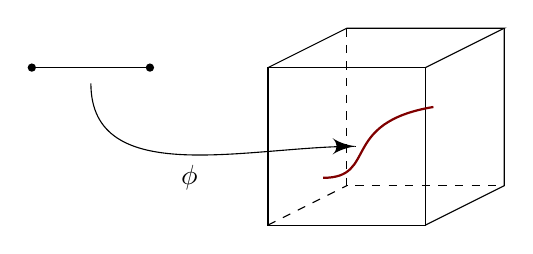
\begin{tikzpicture}
        \draw (0, 0) node [circ] {} -- (1.5, 0) node [circ] {};

        \draw (3, 0) rectangle (5, -2);
        \draw (3, 0) -- (4, 0.5) -- (6, 0.5) -- (5, 0);
        \draw (6, 0.5) -- (6, -1.5) -- (5, -2);
        \draw [dashed] (4, 0.5) -- (4, -1.5) -- (6, -1.5);
        \draw [dashed] (3, -2) -- (4, -1.5);

        \draw (0.75, -0.2) edge [out=270, in=180] (4.1, -1);

        \node at (2, -1.4) {$\phi$};

        \draw [->] (4.099, -1) -- (4.1, -1);

        \draw [thick, mred](3.7, -1.4) .. controls (4.4, -1.4) and (3.9, -0.7) .. (5.1, -0.5);
      \end{tikzpicture}
    \end{center}
    In string theory, we often have fields $\phi: \Sigma \to N$, where $N$ is a \emph{Calabi-Yau manifold}.

    In pion physics, $\pi(x)$ describes a map $\phi: (\R^4, \eta) \to G/H$, where $G$ and $H$ are Lie groups.

    Of course, we can go beyond scalar fields. We can also have fields with non-zero spin such as fermions or gauge fields, eg. a connection on a principal $G$-bundle, as we will figure out later. These are fields that carry a non-trivial representation of the Lorentz group. There is a whole load of things we can choose for our field.

    Whatever field we choose, we let $\mathcal{C}$\index{$\mathcal{C}$} be the space of all field configurations, ie. a point $\phi \in \mathcal{C}$ represents a picture of our field across all of $M$. Thus $\mathcal{C}$ is some form of function space and will typically be infinite dimensional. This infinite-dimensionality is what makes QFT hard, and also what makes it interesting.

  \item We choose an action. An \emph{action} is just a function $S: \mathcal{C} \to \R$. You tell me what the field looks like, and I will give you a number, the value of the action. We often choose our action to be local, in the sense that we assume there exists some function $\mathcal{L}(\phi, \partial \phi, \cdots)$ such that
    \[
      S[\phi] = \int_M\d^4 x \sqrt{g}\; \mathcal{L}(\phi(x), \partial\phi (x), \cdots).
    \]
    The physics motivation behind this choice is obvious --- we don't want what is happening over here to depend on what is happening at the far side of Pluto. However, this assumption is actually rather suspicious, and we will revisit this later.

    For example, we have certainly met actions that look like
    \[
      S[\phi] = \int \d^4 x\; \left(\frac{1}{2} (\partial \phi)^2 + \frac{m^2}{2} \phi^2 + \frac{\lambda}{4!} \phi^4\right),
    \]
    and for gauge fields we might have seen
    \[
      S[A] = \frac{1}{4} \int \d^4 x\; F_{\mu\nu}F^{\mu\nu}.
    \]
    If we have a coupled fermion field, we might have
    \[
      S[A, \psi] = \frac{1}{4} \int \d^4 x\; F_{\mu\nu}F^{\mu\nu} + \bar\psi (\slashed{D} + m) \psi.
    \]
    But recall when we first encountered Lagrangians in classical dynamics, we worked with \emph{lots} of different Lagrangians. We can do whatever thing we like, make the particle roll down the hill and jump into space etc, and we get to deal with a whole family of different Lagrangians. But when we come to quantum field theory, the choices seem to be rather restrictive. Why can't we choose something like
    \[
      S[A] = \int F^2 + F^4 + \cosh(F^2) + \cdots?
    \]
    It turns out we can, and in fact we \emph{must}. We will have to work with something much more complicated.

    But then what were we doing in the QFT course? Did we just waste time coming up with tools that just work with these very specific examples? It turns out not. We will see that there are very good reasons to study these specific actions.
  \item What do we compute? In this course, the main object we'll study is the \term{partition function}
    \[
      \mathcal{Z} = \int_\mathcal{C} \D \phi\; e^{-S[\phi]/\hbar},
    \]
    which is some sort of integral over the space of all fields. Note that the minus sign in the exponential is for the Euclidean signature. If we are not Euclidean, we get some $i$'s instead.

    We will see that the factor of $e^{-S[\phi]/\hbar}$ means that as $\hbar \to 0$, the dominant contribution to the partition function comes from stationary points of $S[\phi]$ over $\mathcal{C}$, and this starts to bring us back to the classical theory of fields. The effect of $e^{-S[\phi]/\hbar}$ is to try to suppress ``wild'' contributions to $\mathcal{Z}$, eg. where $\phi$ is varying very rapidly or $\phi$ takes very large values.

     Heuristically, just as in statistical physics, we have a competition between the two factors $\D \phi$ and $e^{-S[\phi]/\hbar}$. The action part tries to suppress crazy things, but how well this happens depends on how much crazy things are happening, which is measured by the measure $\D \phi$. We can think of this $\D \phi$ as ``entropy''. However, the problem is, the measure $\D \phi$ on $\mathcal{C}$ doesn't actually exist!

    Understanding what we mean by this path integral, and what this measure actually is, and how we can actually compute this thing, and how this has got to do with the canonical quantization operators we had previously, is the main focus of the first part of this course.
\end{enumerate}

\section{QFT in zero dimensions}
We start from the simplest case we can think of, namely quantum field theory in zero dimensions. You might think this is rather trivial, and it is. And this is good.

In $d = 0$, if our universe $M$ is connected, then the only choice of $M$ is $\{\mathrm{pt}\}$. There is a no possibility for a field to have spin, because the Lorentz group is trivial. Our fields are scalar, and the simplest choice is just a single field $\phi: \{\mathrm{pt}\} \to \R$, ie. just a real variable. Similarly, we simply have $\mathcal{C} \cong \R$. This is \emph{not} an infinite-dimensional space.

The action is just a normal function $S: \mathcal{C} \cong \R \to \R$ of one real variable. The path integral measure $\D \phi$ can be taken to just be the standard (Lebesgue) measure $\d \phi$ on $\R$. So our partition function is just
\[
  \mathcal{Z} = \int_\R \d \phi\; e^{-S(\phi)/\hbar},
\]
where we assume $S$ is chosen so that this converges. This happens if $S$ grows sufficiently large as $\phi \to \pm \infty$.

More generally, we may wish to compute \term{correlation functions}, ie. we pick another function $f(\phi)$ and compute the \term{expectation}\index{$\bra f(\phi)\ket$}
\[
  \bra f(\phi)\ket = \frac{1}{\mathcal{Z}} \int \d \phi\; f(\phi) e^{-S(\phi)/\hbar}.
\]
Again, we can pick whatever $f$ we like as long as the integral converges. In this case, $\frac{1}{\mathcal{Z}} e^{-S(\phi)/\hbar}$ is a probability distribution on $\R$, and as the name suggests, $\bra f(\phi)\ket$ is just the expectation value of $f$ in this distribution. Later on, when we study quantum field theory in higher dimensions, we can define more complicated $f$ by evaluating $\phi$ at different points, and we can use this to figure out how the field at different points relate to each other.

Our action is taken to have a series expansion in $\phi$, so in particular we can write
\[
  S(\phi) = \frac{m^2 \phi^2}{2} + \sum_{n = 3}^N g_n \frac{\phi^n}{n!}.
\]
We didn't put in a constant term, as it would just give us a constant factor in $\mathcal{Z}$. We could have included linear terms, but we shall not. The important thing is that $N$ has to be even, so that the asymptotic behaviour of $S$ is symmetric in both sides.

Now the partition function is a function of all these terms: $\mathcal{Z} = \mathcal{Z}(m^2, g_n)$. Similarly, $\bra f\ket$ is again a function of $m^2$ and $g_n$, and possibly other things used to define $f$ itself.

Note that \emph{nothing} depends on the field, because we are integrating over all possible fields.

\subsection{Free theories}
We consider the simplest possible QFT. These QFT's are free, and so $S(\phi)$ is at most quadratic. Classically, this implies the equations of motions are linear, and so there is superposition, and thus the particles do not interact.

Let $\phi: \{\mathrm{pt}\} \to \R^n$ be a field with coordinates $\phi^a$, and define
\[
  S(\phi) = \frac{1}{2} M(\phi, \phi) = \frac{1}{2} M_{ab} \phi^a \phi^b,
\]
where $M: \R^n \times \R^n \to \R$ is a positive-definite symmetric matrix. Then the partition function $\mathcal{Z}(M)$ is just a Gaussian integral:
\[
  \mathcal{Z}(M) = \int_{\R^n} \d^n \phi\; e^{- \frac{1}{2\hbar} M(\phi, \phi)} = \frac{(2 \pi \hbar)^{n/2}}{\sqrt{\det{M}}}.
\]
Indeed, to compute this integral, since $M$ is symmetric, there exists an orthogonal transformation $O: \R^n \to \R^n$ that diagonalizes it. The measure $\d^n \phi$ is invariant under orthogonal transformations. So in terms of the eigenvectors of $M$, this just reduces to a product of $n$ 1D Gaussian integrals of this type, and this is a standard integral:
\[
  \int \d \chi\; e^{-m\chi^2/2\hbar} = \sqrt{\frac{2\pi \hbar}{m}}.
\]
In our case, $m > 0$ runs over all eigenvalues of $M$, and the product of eigenvalues is exactly $\det M$.

A small generalization is useful. We let
\[
  S(\phi) = \frac{1}{2} M(\phi, \phi) + J(\phi),
\]
where $J: \R^n \to \R$ is some linear map (we can think of $J$ as a (co)vector, and also write $J(\phi) = J \cdot \phi$). $J$ is a \emph{source} in the classical case. Then in this theory, we have
\[
  \mathcal{Z}(M, J) = \int_{\R^n} \d^n \phi\; \exp\left(-\frac{1}{\hbar}\left(\frac{1}{2} M(\phi, \phi) + J(\phi)\right)\right).
\]
To do this integral, we complete the square by letting $\tilde{\phi} = \phi + M^{-1}J$. In other words,
\[
  \tilde{\phi}^a = \phi^a + (M^{-1})^{ab} J_b.
\]
The inverse exists because $M$ is assumed to be positive definite. We can now complete the square to find
\begin{align*}
  \mathcal{Z}(M, J) &= \int_{\R^n} \d^n \tilde{\phi} \;\exp\left(\frac{-1}{2\hbar}M(\tilde{\phi}, \tilde{\phi}) + \frac{1}{2\hbar}M^{-1}(J, J)\right)\\
  &= \exp\left(\frac{1}{2\hbar}M^{-1}(J, J)\right)\int_{\R^n} \d^n \tilde{\phi} \;\exp\left(\frac{-1}{2\hbar}M(\tilde{\phi}, \tilde{\phi})\right)\\
  &= \exp\left(\frac{1}{2\hbar}M^{-1}(J, J)\right) \frac{(2\pi \hbar)^{n/2}}{\sqrt{\det M}}.
\end{align*}
In the long run, we really don't care about the case with a source. However, we will use this general case to compute some correlation functions.

We return to the case without a source, and let $P: \R^n \to \R$ be a polynomial. We want to compute
\[
  \bra P(\phi)\ket = \frac{1}{\mathcal{Z}(M)} \int_{\R^n} \d^n \phi\; P(\phi) \exp\left(-\frac{1}{2\hbar} M(\phi, \phi)\right).
\]
By linearity, it suffices to consider the case where $P$ is just a monomial, so
\[
  P(\phi) = \prod_{i = 1}^m (\ell_i(\phi)),
\]
for $\ell_i : \R^n \to \R$ linear maps. Now if $m$ is odd, then clearly $\bra P(\phi)\ket = 0$, since this is an integral of an odd function. When $m = 2k$, then we have
\[
  \bra P(\phi) \ket = \frac{1}{\mathcal{Z}(M)} \int \d^n \phi\; (\ell_i\cdot \phi) \cdots (\ell_{2k} \cdot \phi) \exp\left(-\frac{1}{2\hbar}M (\phi, \phi) - \frac{J \cdot \phi}{\hbar}\right).
\]
Here we are eventually going to set $J = 0$, but for the time being, we will be silly and put the source there. The relevance is that we can then think of our factors $\ell_i \cdot \phi$ as derivatives with respect to $J$:
\begin{align*}
  \bra P(\phi)\ket &= \frac{(-\hbar)^{2k}}{\mathcal{Z}(M)} \int \d^n \phi \; \prod_{i = 1}^{2k} \left(\ell_i \cdot \frac{\partial}{\partial J}\right) \exp\left(-\frac{1}{2\hbar} M(\phi, \phi) - \frac{J\cdot \phi}{\hbar}\right)\\
  \intertext{Since the integral is absolutely convergent, we can move the derivative out of the integral, and get}
  &= \frac{(-\hbar)^{2k}}{\mathcal{Z}(M)} \prod_{i = 1}^{2k} \left(\ell_i \cdot \frac{\partial}{\partial J}\right) \int \d^n \phi \; \exp\left(-\frac{1}{2\hbar} M(\phi, \phi) - \frac{J\cdot \phi}{\hbar}\right)\\
  &= \hbar^{2k} \prod_{i = 1}^{2k} \left(\ell_i \cdot \frac{\partial}{\partial J}\right) \exp\left(\frac{1}{2\hbar}M^{-1}(J, J)\right).
\end{align*}
When each derivative $\ell_i \cdot \frac{\partial}{\partial J}$ acts on the exponential, we obtain a factor of
\[
  \frac{1}{\hbar} M^{-1}(J, \ell_i).
\]
in front. At the end, we are going to set $J = 0$. So we only get contributions if and only if exactly half (ie. $k$) of the derivatives act on the exponential, and the other $k$ act on the factor in front to get rid of the $J$.

We let $\sigma$ denote a (complete) pairing of the set $\{1, \cdots, 2k\}$, and $\Pi_{2k}$ be the set of all such pairings. For example, if we have $k = 2$, then the possible pairings are $\{(1, 2), (3, 4)\}$, $\{(1, 3), (2, 4)\}$ and $\{(1, 4), (2, 3)\}$:
\begin{center}
  \begin{tikzpicture}
    \node [circ] at (0, 0) {};
    \node [circ] at (1, 0) {};
    \node [circ] at (1, 1) {};
    \node [circ] at (0, 1) {};
    \draw (0, 0) -- (0, 1);
    \draw (1, 0) -- (1, 1);

    \begin{scope}[shift={(3, 0)}]
      \node [circ] at (0, 0) {};
      \node [circ] at (1, 0) {};
      \node [circ] at (1, 1) {};
      \node [circ] at (0, 1) {};
      \draw (0, 0) -- (1, 0);
      \draw (0, 1) -- (1, 1);
    \end{scope}

    \begin{scope}[shift={(6, 0)}]
      \node [circ] at (0, 0) {};
      \node [circ] at (1, 0) {};
      \node [circ] at (1, 1) {};
      \node [circ] at (0, 1) {};
      \draw (0, 0) -- (1, 1);
      \draw (1, 0) -- (0, 1);
    \end{scope}
  \end{tikzpicture}
\end{center}
In general, we have
\[
  |\Pi_{2k}| = \frac{(2k)!}{2^k k!},
\]
and we have
\begin{thm}[Wick's theorem]\index{Wick's theorem}
  For a monomial
  \[
    P(\phi) = \prod_{i = 1}^{2k} \ell_i(\phi),
  \]
  we have
  \[
    \bra P(\phi)\ket = \hbar^{k}\sum_{\sigma \in \Pi_{2k}} \prod_{i \in \{1, \cdots, 2k\}/\sigma} M^{-1}(\ell_i, \ell_{\sigma(i)}).
  \]
  where the $\{1, \cdots, 2k\}/\sigma$ says we sum over each pair $\{i, \sigma(i)\}$ only once, rather than once for $(i, \sigma(i))$ and another for $(\sigma(i), i)$.
\end{thm}
This is in fact the version of Wick's theorem for this 0d QFT, and $M^{-1}$ plays the role of the propagator.

For example, we have
\[
  \bra \ell_1(\phi), \ell_2(\phi)\ket = \hbar M^{-1} (\ell_1, \ell_2).
\]
We can represent this by the diagram
\begin{center}
  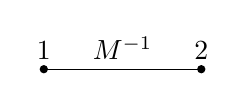
\begin{tikzpicture}
    \node [circ] at (0, 0) {};
    \node [circ] at (2, 0) {};

    \node [above] at (0, 0) {$1$};
    \node [above] at (2, 0) {$2$};
    \draw (0, 0) -- (2, 0) node [pos=0.5, above] {$M^{-1}$};
  \end{tikzpicture}
\end{center}
Similarly, we have
\begin{multline*}
  \bra \ell_1(\phi) \cdots \ell_4(\phi)\ket = \hbar^2 \Big(M^{-1}(\ell_1, \ell_2) M^{-1}(\ell_3, \ell_4) \\
  + M^{-1}(\ell_1, \ell_3) M^{-1}(\ell_2, \ell_4) + M^{-1}(\ell_1, \ell_4) M^{-1}(\ell_2, \ell_3)\Big).
\end{multline*}
This is purely combinatorial.

This is about all we can say for free 0d QFTs. There is an analogue for ``fermions'', which is put in the first example sheet.

\subsection{Interacting theories}
Physically interesting theories contain interactions, ie. $S(\phi)$ is non-quadratic. Typically, if we are trying to compute
\[
  \int \d^n \phi P(\phi) \exp\left(-\frac{S(\phi)}{\hbar}\right),
\]
these things involve transcendental functions and, except in very special circumstances, is just too hard. We usually cannot perform these integrals analytically.

Naturally, in perturbation theory, we would thus want to approximate
\[
  \mathcal{Z} = \int \d^n \phi\; \exp\left(-\frac{S(\phi)}{\hbar}\right)
\]
by some series. Unfortunately, the integral very likely diverges if $\hbar < 0$, as usually $S(\phi) \to \infty$ as $\phi \to \pm\infty$. So it can't have a Taylor series expansion around $\hbar = 0$, as such expansions have to be valid in a disk in the complex plane. The best we can hope for is an asymptotic series.

Recall that a series
\[
  \sum_{n = 0}^\infty f_n(\hbar)
\]
is an \emph{asymptotic series} for $\mathcal{Z}(\hbar)$ if for any fixed $N \in \N$, if we write $\mathcal{Z}_N(\hbar)$ for the first $N$ terms on the RHS, then
\[
  \lim_{\hbar \to 0^+} \frac{|\mathcal{Z}(\hbar) - \mathcal{Z}_N(\hbar)|}{\hbar^N} \to 0.
\]
Thus as $\hbar \to 0^+$, we get an arbitrarily good approximation to what we really wanted from any finite number of terms. But the series will in general diverge if try to fix $\hbar \in \R_{> 0}$, and include increasingly many terms.

Most of the expansions we do in quantum field theories are of this nature.

Now suppose $S(\phi)$ is smooth with a global minimum at $\phi = \phi_0 \in \R^n$, where the Hessian
\[
  \left.\frac{\partial^2 S}{\partial \phi^a \partial \phi^b}\right|_{\phi_0}
\]
is positive definite. Then by Laplace's method/Watson's lemma, we have an asymptotic series of the form
\[
  \mathcal{Z}(\hbar) \sim (2\pi \hbar)^{n/2} \frac{\exp\left(-\frac{S(\phi_0)}{\hbar}\right)}{\sqrt{\det \partial_a \partial_b S(\phi_0)}} \left(1 + A \hbar + B \hbar^2 + \cdots\right).
\]
We will not prove this, but the proof is available in any standard asymptotic methods textbook. The leading term involves the action evaluated on the classical solution $\phi_0$, and is known as the \term{semiclassical term}. Every thing we did last term with tree diagrams was about calculating the first term. The remaining terms are called the \term{quantum correction}.

In Quantum Field Theory last term, the tree diagrams we worked with were just about calculating the leading term. So we weren't actually doing \emph{quantum} field theory (sorry).

\begin{eg}
  Let's consider a single scalar field $\phi$ with action
  \[
    S(\phi) = \frac{m^2}{2}\phi^2 + \frac{\lambda}{4!} \phi^4,
  \]
  where $m^2, \lambda > 0$. The action has a unique global minimum at $\phi_0 = 0$. The action evaluated at $\phi_0 = 0$ vanishes, and $\partial^2 S/\hbar = m^2$. So the leading term in the asymptotic expansion of $\mathcal{Z}(\hbar, m \lambda)$ is
  \[
    \frac{(2\pi \hbar)^{1/2}}{m}.
  \]
  Further, we can find the whole series expansion by
  \begin{align*}
    \mathcal{Z}(\hbar, m, \lambda) &= \int_\R \d \phi \; \exp\left(\frac{-1}{\hbar}\left(\frac{m^2}{2} \phi^2 + \frac{\lambda}{4!}\phi^4\right)\right)\\
    &= \frac{\sqrt{2\hbar}}{m} \int \d \tilde{\phi} \exp\left(-\tilde{\phi}^2 \right) \exp\left( - \frac{4\lambda \hbar}{4! m^4} \tilde{\phi}^4\right)\\
    &\sim \frac{\sqrt{2\hbar}}{m} \int \d \tilde{\phi}\; e^{- \tilde{\phi}^2}\sum_{n = 0}^N \frac{1}{n!} \left(\frac{-\lambda \hbar}{3! m^4}\right)^n \tilde{\phi}^{4n}\\
    &= \frac{\sqrt{2\hbar}}{m} \sum_{n = 0}^N \left(\frac{-\lambda \hbar}{3! m^4}\right)^n \frac{1}{n!} \int \d \tilde{\phi}\;e^{- \tilde{\phi}^2}\tilde{\phi}^{4n}\\
    &= \frac{\sqrt{2\hbar}}{m} \sum_{n = 0}^N \left(\frac{-\lambda \hbar}{3! m^4}\right)^n \frac{1}{n!} \Gamma\left(2n + \frac{1}{2}\right).
  \end{align*}
  The last line uses the definition of the Gamma function.

  We can plug in the value of the $\Gamma$ function to get
  \begin{align*}
    \mathcal{Z}(\hbar, m \lambda) &\sim \frac{\sqrt{2\hbar \pi}}{m} \sum_{n = 0}^N \left(\frac{-\hbar \lambda}{m^4}\right)^n \frac{1}{(4!)^n n!} \frac{(4n)!}{4^n (2n)!}\\
    &= \frac{\sqrt{2\pi \hbar}}{m} \left(1 - \frac{\hbar\lambda}{8m^4} + \frac{35}{384} \frac{\hbar^2 \lambda^2}{m^8} + \cdots\right).
  \end{align*}
  We will get to understand these coefficients much more in terms of Feynman diagrams later.

  Note that up to the factor $\frac{\sqrt{2\pi \hbar}}{m}$, the series depends on $(\hbar, \lambda)$ only through the product $\hbar \lambda$. So we can equally view it as an asymptotic series in the coupling constant $\lambda$.
\end{eg}
As we emphasized previously, we get an asymptotic series, not a Taylor series. Why is this so?

When we first started our series expansion, we wrote $\exp(-S(\phi)/\hbar)$ as a series in $\lambda$. This is absolutely fine, as $\exp$ is a very well-behaved function when it comes to power series. The problem comes when we want to interchange the integral with the sum. We know this is allowed only if the sum is absolutely convergent, but it is not, as the integral does not converge for negative $\hbar$. Thus, the best we can do is that for any $N$, we truncate the sum at $N$, and then do the exchange. This is legal since finite sums always commute with integrals.

We can in fact see the divergence of the asymptotic series for finite $(\hbar \lambda) > 0$ from the series itself, using Stirling's approximation. Recall we have
\[
  n! \sim e^{n \log n}.
\]
So via a straightforward manipulation, we have
\[
  \frac{1}{(4!)^n n!} \frac{(4n)!}{4^n(2n)!} \sim e^{n \log n}.
\]
So the coefficients go faster than exponentially, and thus the series has vanishing radius of convergence.

We can also see other weird phenomena here. Suppose we decided that we have $m^2 < 0$ instead (which is a rather weird thing to do). Then it is clear that $\mathcal{Z}(m^2, \lambda)$ still exists, as the $\phi^4$ eventually dominates, and so what happens at the $\phi^2$ term doesn't really matter. However, the asymptotic series is invalid in this region.

Indeed, if we look at the fourth line of our derivation, each term in the asymptotic series will be obtained by integrating $e^{\tilde\phi^2} \tilde\phi^{4n}$, instead of integrating $e^{-\tilde\phi^2} \tilde\phi^{4n}$, and each of these integrals would diverge.

Fundamentally, this is since when $m^2 < 0$, the global minimum of $S(\phi)$ are now at
\[
  \phi_0 = \pm \sqrt{\frac{6m^2}{\lambda}}.
\]
\begin{center}
  \begin{tikzpicture}
    \draw [->](-3, 0) -- (3, 0) node [right] {$\phi$};
    \draw [->] (0, -1.2) -- (0, 3) node [above] {$S(\phi)$};

    \draw [mblue, thick, domain=-2.4:2.4, samples=50] plot [smooth] (\x, {4 * ((\x/2)^4 - (\x/2)^2)});

    \draw [dashed] (1.414, 0) node [above] {$\phi_0$} -- (1.414, -1);
  \end{tikzpicture}
\end{center}
Our old minimum $\phi = 0$ is now a (local) maximum!T This is the wrong point to expand about! Fields with $m^2 < 0$ are called \term{tachyons}, and these are always signs of some form of instability.

Actions whose minima occur at non-zero field values are often associated with \term{spontaneous symmetry breaking}. Our original theory has a $\Z/2$ symmetry, namely under the transformation $x \leftrightarrow -x$. But once we pick a minimum $\phi_0$ to expand about, we have broken the symmetry. This is an interesting kind of symmetry breaking because the asymmetry doesn't really exist in our theory. It's just our arbitrary choice that breaks it.

\subsection{Feynman diagrams}
We now try to understand the terms in the asymptotic series in terms of Feynman diagrams. The easy bits are the powers of
\[
  \left(\frac{\hbar \lambda}{m^4}\right)^n.
\]
This combination is essentially fixed by dimensional analysis. What we really want to understand are the combinatorial factors, given by
\[
  \frac{1}{(4!)^n n!} \times \frac{(4n)!}{4^n (2n)!}.
\]
The first factor just came from expanding $\exp(-\lambda \phi^4/4!)$ in the exponential. The second term is more interesting. It is the number of ways of joining $4n$ elements into inequivalent pairs. This is something we saw when we looked at Wick's theorem. We have $4n$ instead of $2n$ because we are now doing perturbation theory with $\phi^4$, not $\phi^2$.

We now try to come up with some Feynman diagrams to represent our asymptotic series. We have a single type of propagator that looks like this:
\begin{center}
  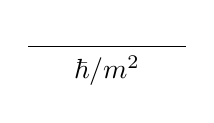
\begin{tikzpicture}
    \draw (0, 0) -- (2, 0) node [pos=0.5, below] {$\hbar/m^2$} node [pos=0.5, above] { };
  \end{tikzpicture}
\end{center}
and we also have a vertex
\begin{center}
  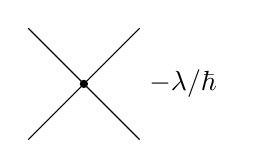
\begin{tikzpicture}[scale=0.707]
    \draw (0, 0) -- (2, 2);
    \draw (0, 2) -- (2, 0);
    \node [circ] at (1, 1) {};
    \node [right] at (2, 1) {$-\lambda /\hbar$};
  \end{tikzpicture}
\end{center}
The negative sign appears because we have $e^{-S}$ in ``Euclidean'' QFT.

Since we are computing just the partition functions, we want to try to find all \term{vacuum graphs}, ie. graphs with no external edges. The only allowed components are the propagator and vertices.

At order $\lambda$, we have
\begin{center}
  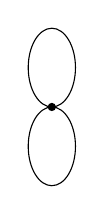
\begin{tikzpicture}
    \node [circ] at (0, 0) {};

    \draw (0, 0.5) ellipse (0.3 and 0.5);
    \draw (0, -0.5) ellipse (0.3 and 0.5);
  \end{tikzpicture}
\end{center}
For our purposes, it is useful to consider the four outgoing vertices of the diagram as sort-of distinct. So the following can be considered different diagrams:
\begin{center}
  \makecenter{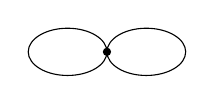
\begin{tikzpicture}
    \node [circ] at (0, 0) {};

    \draw (0.5, 0) ellipse (0.5 and 0.3);
    \draw (-0.5, 0) ellipse (0.5 and 0.3);
  \end{tikzpicture}}
  \quad
  \makecenter{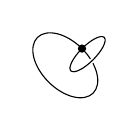
\begin{tikzpicture}[rotate=135]
    \draw (0, 0.3) ellipse (0.5 and 0.3);
    \draw [ultra thick, white] (-0.1, 0) ellipse (0.1 and 0.3);
    \draw (-0.1, 0) ellipse (0.1 and 0.3);

    \node [circ] at (0, 0) {};
  \end{tikzpicture}}
\end{center}
However, we will say these are \emph{topologically equivalent}. In the future, we will count these as the ``same'' diagram, and only include them once in the series expansion, but we will later see the need to distinguish between them when we want to figure out how many times we count each diagram.

In terms of these diagrams, we can write
\[\arraycolsep=0.25em\def\arraystretch{2.2}
  \begin{array}{ccccccccccccc}
  \displaystyle\frac{\mathcal{Z}(m^2, \lambda)}{\mathcal{Z}(m^2, 0)} & \sim &
  \begin{tikzpicture}[eqpic]
    \node {$\emptyset$};
  \end{tikzpicture} &+&
  \begin{tikzpicture}[eqpic]
    \node [circ] at (0, 0) {};

    \draw (0, 0.5) ellipse (0.3 and 0.5);
    \draw (0, -0.5) ellipse (0.3 and 0.5);
  \end{tikzpicture}
  &+&
  \begin{tikzpicture}[eqpic]
    \node [circ] at (0, 0) {};
    \node [circ] at (1.5, 0) {};
    \draw (0.75, 0) ellipse (0.75 and 0.7);
    \draw (0.75, 0) ellipse (0.75 and 0.4);
  \end{tikzpicture}
  &+&
  \begin{tikzpicture}[eqpic]
    \node [circ] at (0, 0) {};
    \node [circ] at (1, 0) {};
    \draw (-0.2, 0) ellipse (0.2 and 0.5);
    \draw (0.5, 0) ellipse (0.5 and 0.3);
    \draw (1.2, 0) ellipse (0.2 and 0.5);
  \end{tikzpicture}
  &+&
  \begin{tikzpicture}[eqpic]
    \node [circ] at (0, 0) {};

    \draw (0, 0.5) ellipse (0.3 and 0.5);
    \draw (0, -0.5) ellipse (0.3 and 0.5);

    \node [circ] at (0.7, 0) {};

    \draw (0.7, 0.5) ellipse (0.3 and 0.5);
    \draw (0.7, -0.5) ellipse (0.3 and 0.5);
  \end{tikzpicture}
  &+&
  \cdots\\
  && 1 &+& \displaystyle\frac{-\lambda \hbar}{m^4} \frac{1}{8} &+& \displaystyle\frac{\lambda^2 \hbar^2}{m^8} \frac{1}{48} &+& \displaystyle\frac{\lambda^2 \hbar^2}{m^8} \frac{1}{16} &+& \displaystyle\frac{\lambda^2 \hbar^2}{m^8} \frac{1}{128} &+& \cdots
\end{array}
\]
The $\lambda, \hbar$ and $m$ factors just come directly form the Feynman rules, but where did the numerical factors come from?

Let $D_n$ be the set of all Feynman graphs with $n$ vertices. By some combinatorics, we find that there are
\[
  |D_n| = \frac{(4n)!}{4^n (2n)!}
\]
of these. For example, $|D_1| = 3$, as we have previously seen listed.

This set $D_n$ is acted on by a group $G_n = (S_4)^n \rtimes S_n$, where $S_4$ permutes the $4$ loops on a given vertex, and $S_n$ permutes the different vertices. The order of this group is
\[
  |G_n| = (4!)^n n!
\]
Then we see that our asymptotic series can be written as
\[
  \frac{\mathcal{Z}(m^2, \lambda)}{\mathcal{Z}(m^2, 0)} \sim \sum_{n = 0}^N \frac{|D_n|}{|G_n|} \left(\frac{-\hbar \lambda}{m^4}\right)^n.
\]
Now we just gave names to these numbers, and it doesn't help us actually compute them from Feynman diagrams. To make more sense of these numbers, we need to use the renowned \emph{orbit-stabilizer theorem} we learnt from IA Groups.

Note that when $G_n$ acts on $D_n$, the action does not change the topology of the graph, ie. after the action of $G_n$, the graph is still topologically equivalent to the original one. In particular, the set of \term{orbits} $\mathcal{O}_N$ of $D_n$ under the $G_n$-action are exactly the topologically distinct graphs.

For example, we have $|\mathcal{O}_1| = 1$ and $|\mathcal{O}_2| = 3$.

Now we fix a particular element $\Gamma \in G_n$, and pick one particular graph that represents $\Gamma$, say
\begin{center}
  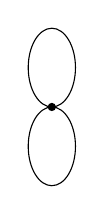
\begin{tikzpicture}
    \node [circ] at (0, 0) {};

    \draw (0, 0.5) ellipse (0.3 and 0.5);
    \draw (0, -0.5) ellipse (0.3 and 0.5);
  \end{tikzpicture}
\end{center}
Now if we swap the two top legs, then we get back the same graph. However, if we swap the top-right and bottom-left legs, we end up with
\begin{center}
  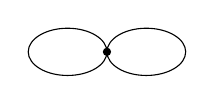
\begin{tikzpicture}
    \node [circ] at (0, 0) {};

    \draw (0.5, 0) ellipse (0.5 and 0.3);
    \draw (-0.5, 0) ellipse (0.5 and 0.3);
  \end{tikzpicture}
\end{center}
We write $\Aut \Gamma$ for the set (and in fact subgroup) of all elements in $G_n$ that preserve the graph. It is an easy exercise to show this does not depend which representative of $\Gamma$ we pick. This is known as the \term{stabilizer} of $\Gamma$.

Now by the \term{orbit-stabilizer theorem}, we know
\[
  \frac{|D_n|}{|G_n|} = \sum_{\Gamma \in \mathcal{O}_n} \frac{1}{|\Aut\Gamma|}.
\]
For example, in $n = 1$, the graph
\begin{center}
  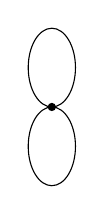
\begin{tikzpicture}
    \node [circ] at (0, 0) {};

    \draw (0, 0.5) ellipse (0.3 and 0.5);
    \draw (0, -0.5) ellipse (0.3 and 0.5);
  \end{tikzpicture}
\end{center}
has stabilizer of size $8$. This is generated by swapping the top legs; swapping the bottom legs; and a vertical flip.

In $n = 2$, the graph
\begin{center}
  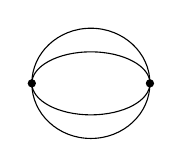
\begin{tikzpicture}
    \node [circ] at (0, 0) {};
    \node [circ] at (1.5, 0) {};
    \draw (0.75, 0) ellipse (0.75 and 0.7);
    \draw (0.75, 0) ellipse (0.75 and 0.4);
  \end{tikzpicture}
\end{center}
has $|\Aut \Gamma| = 4! \times 2 = 48$, as we can permute any of the edges, giving a factor of $4!$, and we can also swap around the two vertices.

In
\begin{center}
  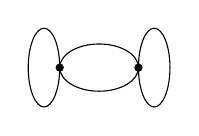
\begin{tikzpicture}
    \node [circ] at (0, 0) {};
    \node [circ] at (1, 0) {};
    \draw (-0.2, 0) ellipse (0.2 and 0.5);
    \draw (0.5, 0) ellipse (0.5 and 0.3);
    \draw (1.2, 0) ellipse (0.2 and 0.5);
  \end{tikzpicture}
\end{center}
we have $|\Aut\Gamma| = 2^3 \times 2 = 16$, as we can flip the left; middle; or right loops, giving $2^3$, and also we can flip the whole thing around horizontally.

Finally, in
\begin{center}
  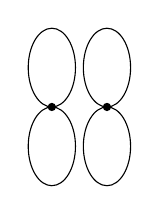
\begin{tikzpicture}
    \node [circ] at (0, 0) {};

    \draw (0, 0.5) ellipse (0.3 and 0.5);
    \draw (0, -0.5) ellipse (0.3 and 0.5);

    \node [circ] at (0.7, 0) {};

    \draw (0.7, 0.5) ellipse (0.3 and 0.5);
    \draw (0.7, -0.5) ellipse (0.3 and 0.5);
  \end{tikzpicture}
\end{center}
we have $|\Aut\Gamma| = 8 \times 8 \times 2 = 128$, as we have $8$ on each individual component, and we can also swap them.

More generally, if we have a theory with several fields with propagators of value $\frac{1}{P_i}$, and many different interactions with coupling constants $\lambda_\alpha$, then
\[
  \frac{\mathcal{Z}(\lambda_\alpha)}{ \mathcal{Z}(0)} = \sum_{n = 0}^N \sum_{\Gamma \in \mathcal{O}_N} \frac{1}{|\Aut \Gamma|} \frac{\prod_\alpha \lambda_\alpha^{|v_\alpha(\Gamma)|}}{\prod_i |P_i|^{|e_i(\Gamma)|}} \hbar^{E(\Gamma) - V(\Gamma)},
\]
where
\begin{itemize}
  \item $e_i(\Gamma)$ is the number of edges of type $i$ in $\Gamma$;
  \item $v_\alpha(\Gamma)$ is the number of vertices of type $\alpha$ in $\Gamma$;
  \item $V(\Gamma)$ is the number of vertices in total; and
  \item $E(\Gamma)$ the total number of edges.
\end{itemize}
But by Euler's theorem, we have $E - V = L - C$, where $L$ is the number of loops in the graph and $C$ is the number of connected components. So we can also write the factor as $\hbar^{L - C}$.

Finally, note that
\[
  \log (\mathcal{Z}/\mathcal{Z}_0)
\]
is the sum of all \emph{connected} graphs. Indeed, we can see that the term for the two-figure-of-eight is just the square of the term for a single figure-of-eight times the factor of $\frac{1}{2!}$, and one can easily convince oneself that this is true for any number of disconnected sums.

In general, A generic QFT has an asymptotic series
\[
  \mathcal{Z}(\hbar) \sim (2\pi \hbar)^{n/2}\frac{e^{-S(\phi_0)/\hbar}}{\sqrt{ \det \partial \partial S|_{\phi_0}}} (1 + a_1 \hbar + a_2 \hbar^2 + \cdots),
\]
and the terms in the series can be computed by Feynman diagrams.

In some special theories, the leading term is the \emph{exact} answer! The tail terms somehow manage to cancel each other out. This happens for supersymmetry theories. We will not go into the exact details.

\subsection{An effective theory}
We now play with another toy theory. Suppose we have two scalar fields $\phi, \chi \in \R$, and consider the action
\[
  S(\phi, \chi) = \frac{m^2}{2}\phi^2 + \frac{M^2}{2} \chi^2 + \frac{\lambda}{4} \phi^2 \chi^2.
\]
Correspondingly, we have Feynman rules
\begin{center}
  \makecenter{
  \begin{tikzpicture}
    \draw (0, 0) -- (2, 0) node [pos=0.5, below] {$1/m^2$} node [pos=0.5, above] { };
  \end{tikzpicture}}\quad\quad
  \makecenter{\begin{tikzpicture}
    \draw [dashed] (0, 0) -- (2, 0) node [pos=0.5, below] {$1/M^2$} node [pos=0.5, above] { };
  \end{tikzpicture}}
\end{center}
with a vertex
\begin{center}
  \begin{tikzpicture}[scale=0.707]
    \draw (0, 0) -- (2, 2);
    \draw [dashed] (0, 2) -- (2, 0);
    \node [circ] at (1, 1) {};
    \node [right] at (2, 1) {$-\lambda$};
  \end{tikzpicture}
\end{center}
We can use these to compute correlation functions and expectation values.
For example, we might want to compute
\[
  \log (\mathcal{Z}/\mathcal{Z}_0).
\]
We have a diagram that looks like
\[\everymath{\displaystyle}\arraycolsep=0.17em\def\arraystretch{2.2}
  \begin{array}{ccccccccccc}
  \displaystyle\log \left(\frac{\mathcal{Z}(m^2, \lambda)}{\mathcal{Z}(m^2, 0)}\right) & \sim &
  \begin{tikzpicture}[eqpic]
    \node [circ] at (0, 0) {};

    \draw [dashed] (0, 0.5) ellipse (0.3 and 0.5);
    \draw (0, -0.5) ellipse (0.3 and 0.5);
  \end{tikzpicture}
  &+&
  \begin{tikzpicture}[eqpic]
    \node [circ] at (0, 0) {};
    \node [circ] at (1, 0) {};
    \draw (-0.2, 0) ellipse (0.2 and 0.5);
    \draw [dashed] (0.5, 0) ellipse (0.5 and 0.3);
    \draw (1.2, 0) ellipse (0.2 and 0.5);
  \end{tikzpicture}
  &+&
  \begin{tikzpicture}[eqpic]
    \node [circ] at (0, 0) {};
    \node [circ] at (1, 0) {};
    \draw [dashed] (-0.2, 0) ellipse (0.2 and 0.5);
    \draw (0.5, 0) ellipse (0.5 and 0.3);
    \draw [dashed] (1.2, 0) ellipse (0.2 and 0.5);
  \end{tikzpicture}
  &+&
  \begin{tikzpicture}[eqpic]
    \node [circ] at (0, 0) {};
    \node [circ] at (1.5, 0) {};
    \draw [dashed] (0.75, 0) ellipse (0.75 and 0.7);
    \draw (0.75, 0) ellipse (0.75 and 0.4);
  \end{tikzpicture}
  &+&
  \cdots\\
  && \frac{-\lambda}{4m^2 M^2} &+& \frac{\lambda^2}{16 m^4 M^4} &+& \frac{\lambda^2}{16 m^4 M^4} &+& \frac{\lambda^2}{8 m^4 M^4} &+& \cdots\\
\end{array}
\]
We can also try to compute $\bra \phi^2\ket$. To do so, we consider diagrams with two vertices connected to a solid line:
\begin{center}
  \begin{tikzpicture}
    \draw (0, 0) node [circ] {} -- (2, 0);
  \end{tikzpicture}
\end{center}
The relevant diagrams are
\[\everymath{\displaystyle}\arraycolsep=0.3em\def\arraystretch{2.2}
  \begin{array}{ccccccccccccc}
  \displaystyle \bra \phi^2 \ket &\sim&
  \begin{tikzpicture}[eqpic]
    \node [circ] at (0, 0) {};
    \node [circ] at (0, -2) {};
    \draw (0, 0) -- (0, -2);
  \end{tikzpicture}
  &+&
  \begin{tikzpicture}[eqpic]
    \node [circ] at (0, 0) {};
    \node [circ] at (0, -2) {};
    \draw (0, 0) -- (0, -2);

    \node [circ] at (0, -1) {};

    \draw [dashed] (0.4, -1) ellipse (0.4 and 0.25);
  \end{tikzpicture}
  &+&
  \begin{tikzpicture}[eqpic]
    \node [circ] at (0, 0) {};
    \node [circ] at (0, -2) {};
    \draw (0, 0) -- (0, -2);

    \node [circ] at (0, -0.667) {};
    \node [circ] at (0, -1.333) {};

    \draw [dashed] (0.4, -0.667) ellipse (0.4 and 0.25);
    \draw [dashed] (0.4, -1.333) ellipse (0.4 and 0.25);
  \end{tikzpicture}
  &+&
  \begin{tikzpicture}[eqpic]
    \node [circ] at (0, 0) {};
    \node [circ] at (0, -2) {};
    \draw (0, 0) -- (0, -2);

    \node [circ] at (0, -0.667) {};
    \node [circ] at (0, -1.333) {};

    \draw [dashed] (0, -1) ellipse (0.333 and 0.333);
  \end{tikzpicture}
  &+&
  \begin{tikzpicture}[eqpic]
    \node [circ] at (0, 0) {};
    \node [circ] at (0, -2) {};
    \draw (0, 0) -- (0, -2);
    \node [circ] at (0, -1) {};

    \draw [dashed] (0.4, -1) ellipse (0.4 and 0.25);
    \node [circ] at (0.8, -1) {};

    \draw (1.2, -1) ellipse (0.4 and 0.25);
  \end{tikzpicture}
  &+&
  \cdots\\
  && \frac{1}{m^2} &+& \frac{-\lambda}{2m^4 M^4} &+& \frac{\lambda^2}{4m^6 M^4} &+& \frac{\lambda^2}{2m^6 M^4} &+& \frac{\lambda^2}{4m^6 M^4} &+& \cdots\\
\end{array}
\]
Let's arrive at this result in a different way. Suppose we think of $\chi$ as ``heavy'', so we cannot access it directly using our experimental equipment. In particular, if we're only interested in the correlation functions that depend only on $\phi$, then we could try to ``integrate out'' $\chi$ first.

Suppose we have a function $f(\phi)$, and consider the integral
\[
  \int_{\R^2} \d \phi\;\d \chi\; f(\phi) e^{-S(\phi, \chi)/\hbar} = \int_\R \d \phi \left(f(\phi) \int_\R \d \chi\;e^{-S(\phi, \chi)/\hbar}\right).
\]
We define the \term{effective action} for $\phi$, $S_{\mathrm{eff}}(\phi)$ by
\[
  S_{\mathrm{eff}}(\phi) = -\hbar \log \left(\int_\R \d \chi e^{-S(\phi, \chi)/\hbar}\right).
\]
Then the above integral becomes
\[
  \int_\R \d \phi\; f(\phi) e^{-S_{\mathrm{eff}}(\phi)/\hbar}.
\]
So doing any computation with $\phi$ only is equivalent to pretending $\chi$ doesn't exist, and using this effective potential instead.


In general, the integral is very difficult to compute, and we can only find an asymptotic series for the effective action. However, in this very particular example, we have chosen $S$ such that it is only quadratic in $\chi$, and one can compute to get
\[
  \int_\R \d \chi\; e^{-S(\phi, \chi)/\hbar} = e^{-m^2 \phi^2/2\hbar} \sqrt{\frac{2\pi \hbar}{M^2 + \lambda \phi^2/2}}.
\]
Therefore we have
\begin{align*}
  S_{\mathrm{eff}}(\phi) &= \frac{m^2}{2}\phi^2 + \frac{\hbar}{2} \log \left(1 + \frac{\lambda \phi^2}{2M^2}\right) + \frac{\hbar}{2} \log \left(\frac{M^2}{2\pi \hbar}\right)\\
  &= \left(\frac{m^2}{2} + \frac{\hbar \lambda}{4M^2}\right)\phi^2 - \frac{\hbar \lambda^2}{16 M^4} \phi^4 + \frac{\hbar \lambda^3}{48 M^6} \phi^6 + \cdots + \frac{\hbar}{2} \log \left(\frac{M^2}{2\pi \hbar}\right)\\
  &= \frac{m_{\mathrm{eff}}^2}{2} \phi^2 + \frac{\lambda_4}{4!} \phi^4 + \frac{\lambda_6}{6!} \phi^6 + \cdots + \frac{\hbar}{2} \log \left(\frac{M^2}{2\pi \hbar}\right),
\end{align*}
where
\[
  \lambda_{2k} = (-1)^{k + 1} \frac{\hbar (2k)!}{2^{k + 1}k!} \frac{\lambda^k}{M^{2k}}.
\]
We see that once we integrated out $\chi$, we have generated an \emph{infinite series} of new interactions for $\phi$ in $S_{\mathrm{eff}} (\phi)$. Moreover, the mass also shifted as
\[
  m^2 \mapsto m^2_{\mathrm{eff}} = m^2 + \frac{\hbar \lambda}{2M^4}.
\]
Notice the new vertices generated are \emph{quantum effects}. They vanish as $\hbar \to 0$ (they happen to be linear in $\hbar$ here, but that is just a coincidence). They are also suppressed by powers of $\frac{1}{M^2}$. So if $\chi$ is very very heavy, we might think these new couplings have very tiny effects.

This is a very useful technique. If the universe is very complicated with particles at very high energies, then it would be rather hopeless to try to account for all of the effects of the particles we cannot see. In fact, it is impossible to know about these very high energy particles, as their energy are too hight to reach. All we can know about them is their incarnation in terms of these induced couplings on lower energy fields.

A few things to note:
\begin{itemize}
  \item The original action had a $\Z_2 \times \Z_2$ symmetry, given by $(\phi, \chi) \mapsto (\pm \phi, \pm \chi)$. This symmetry is preserved, and we do not generate any vertices with odd powers of $\phi$.
  \item The field $S_{\mathrm{eff}}(\phi)$ also contains a field independent term
    \[
      \frac{\hbar}{2} \log \left(\frac{M^2}{2\pi \hbar}\right).
    \]
    This plays no role in correlation functions $\bar f(\phi)\ket$. Typically, we are just going to drop it. However, this is one of the biggest problem in physics. This term contributes to the cosmological constant, and the values we typically obtain is much larger than the actual observed cosmological constant, and there is no reason to expect that these constants magically cancel out.
  \item In this case, passing to the effective action produced a lot of \emph{new} interactions. However, if we already had a complicated theory, eg. when we started off with an effective action, and then decided to integrate out more things, then instead of introducing new interactions, the effect of this becomes \emph{shifting} the coupling constants, just as we shifted the mass term.
\end{itemize}

In general, how can we compute the effective potential? We are still computing an integral of the form
\[
  \int_\R \d \chi\; e^{-S(\phi, \chi)/\hbar},
\]
so our previous technique of using Feynman diagrams should still work. We will treat $\phi$ as a constant in the theory. So instead of having a vertex that looks like
\begin{center}
  \begin{tikzpicture}[scale=0.707]
    \draw (0, 0) -- (2, 2);
    \draw [dashed] (0, 2) -- (2, 0);
    \node [circ] at (1, 1) {};
    \node [right] at (2, 1) {$-\lambda$};
  \end{tikzpicture}
\end{center}
we drop all the $\phi$ lines and are left with
\begin{center}
  \begin{tikzpicture}[scale=0.707]
    \draw [dashed] (0, 2) -- (2, 0);
    \node [circ] at (1, 1) {};
    \node [right] at (2, 1) {$-\lambda \phi^2$};
  \end{tikzpicture}
\end{center}
But actually, this would be rather confusing. So instead what we do is that we still draw the solid $\phi$ lines, but whenever such a line appears, we have to terminate the line immediately, and this contributes a factor of $\phi$:
\begin{center}
  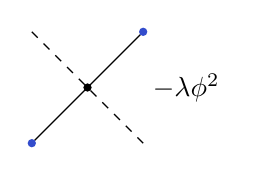
\begin{tikzpicture}[scale=0.707]
    \draw (0, 0) node [circ, mblue] {} -- (2, 2) node [circ, mblue] {};
    \draw [dashed] (0, 2) -- (2, 0);
    \node [circ] at (1, 1) {};
    \node [right] at (2, 1) {$-\lambda \phi^2$};
  \end{tikzpicture}
\end{center}
For our accounting purposes, we will say the internal vertex contributes a factor of $-\lambda$, and each terminating blue vertex contributes a factor of $\phi$.

Since we have a ``constant'' term $\frac{m^2}{2} \phi^2$ as well, we need to add one more diagram to account for that. We allow a single edge of the form
\begin{center}
  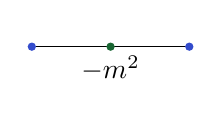
\begin{tikzpicture}
    \draw (0, 0) node [mblue, circ] {} -- (2, 0) node [mblue, circ] {} node [pos=0.5, below] {$-m^2$} node [pos=0.5, above] { };
    \node [circ, mgreen] at (1, 0) {};
  \end{tikzpicture}
\end{center}
With these ingredients, we can compute the effective potential as follows:
\[\everymath{\displaystyle}\arraycolsep=0.3em\def\arraystretch{2.2}
  \begin{array}{ccccccccccc}
    \displaystyle -S_{\mathrm{eff}}(\phi) &\sim&
  \begin{tikzpicture}[eqpic]
    \node [circ, mblue] at (0, 0) {};
    \node [circ, mblue] at (0, -2) {};
    \draw (0, 0) -- (0, -2);
  \end{tikzpicture}
  &+&
  \begin{tikzpicture}[eqpic]
    \node [circ, mblue] at (0, 0) {};
    \node [circ, mblue] at (0, -2) {};
    \draw (0, 0) -- (0, -2);

    \node [circ] at (0, -1) {};

    \draw [dashed] (0.4, -1) ellipse (0.4 and 0.25);
  \end{tikzpicture}
  &+&
  \begin{tikzpicture}[eqpic]
    \draw (0, 0) node [circ, mblue] {} -- +(0, -1) node [circ] {} -- +(0, -2) node [circ, mblue] {};
    \draw (0.8, 0) node [circ, mblue] {} -- +(0, -1) node [circ] {} -- +(0, -2) node [circ, mblue] {};
    \draw [dashed] (0.4, -1) ellipse (0.4 and 0.25);
  \end{tikzpicture}
  &+&
  \begin{tikzpicture}[eqpic]
    \draw (0, 0) node [circ, mblue] {} -- +(0, -1) node [circ] {} -- +(0, -2) node [circ, mblue] {};
    \draw (0.8, 0) node [circ, mblue] {} -- +(0, -1) node [circ] {} -- +(0, -2) node [circ, mblue] {};
    \draw (0.4, 0.25) node [circ, mblue] {} -- +(0, -1) node [circ] {} -- +(0, -2) node [circ, mblue] {};
    \draw [dashed] (0.4, -1) ellipse (0.4 and 0.25);
  \end{tikzpicture}
  &+&
  \cdots\\
  && \frac{-m^2}{2}\phi^2 &+& \frac{-\lambda}{4 M^2} \phi^2 &+& \frac{\lambda^2 \phi^4}{16 M^4} &+& \frac{- \lambda^3 \phi^6}{48 M^6} &+& \cdots
\end{array}
\]
These are just the terms we've previously found. There are, again, a few things to note
\begin{itemize}
  \item The diagram expansion is pretty straightforward in this case, because we started with a rather simple interacting theory. More complicated examples will have diagram expansions that are actually interesting.
  \item We only sum over connected diagrams, as $S_{\mathrm{eff}}$ is the logarithm of the integral.
  \item We see that the new/shifted couplings in $S_{\mathrm{eff}} (\phi)$ are generated by \emph{loops} of $\chi$ fields.
\end{itemize}

\begin{eg}
  We can use the effective potential to compute $\bar \phi^2 \ket$:
  \[\everymath{\displaystyle}\arraycolsep=0.3em\def\arraystretch{2.2}
    \begin{array}{ccccccc}
      \displaystyle \bra \phi^2 \ket &\sim&
      \begin{tikzpicture}[eqpic]
        \node [circ] at (0, 0) {};
        \node [circ] at (0, -2) {};
        \draw (0, 0) -- (0, -2);
      \end{tikzpicture}
      &+&
      \begin{tikzpicture}[eqpic]
        \node [circ] at (0, 0) {};
        \node [circ] at (0, -2) {};
        \draw (0, 0) -- (0, -2);

        \node [circ] at (0, -1) {};

        \draw (0.4, -1) ellipse (0.4 and 0.25);
      \end{tikzpicture}
      &+&
      \cdots\\
      && \frac{1}{m_{\mathrm{eff}}^2} &+& \frac{-\lambda}{2m^6_{\mathrm{eff}}} &+& \cdots
    \end{array}
  \]
  We can see that this agrees with our earlier calculation correct to order $\lambda^2$.
\end{eg}

At this moment, this is not incredibly impressive, since it takes a lot of work to compute $S_{\mathrm{eff}}(\phi)$. But the computation of $S_{\mathrm{eff}}(\phi)$ can be reused to compute any correlation involving $\phi$. So if we do many computations with $\phi$, then we we can save time.

But the point is not that this saves work. The point is that this is what we do when we do physics. We \emph{have} to do this if we don't really know anything about $\chi$, but we can try to figure out $S_{\mathrm{eff}}(\phi^2)$ by working with experiments.

\section{QFT in one dimension (ie. QM)}
\subsection{Quantum mechanics}
In $d = 1$, there are two possible connected, compact manifolds $M$ --- we can have $M = S^1$ or $M = I = [0, 1]$.
\begin{center}
  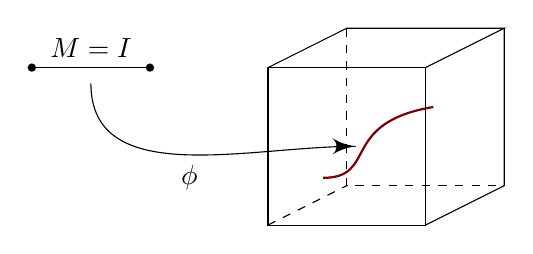
\begin{tikzpicture}
    \draw (0, 0) node [circ] {} -- (1.5, 0) node [circ] {} node [pos=0.5, above] {$M = I$};

    \draw (3, 0) rectangle (5, -2);
    \draw (3, 0) -- (4, 0.5) -- (6, 0.5) -- (5, 0);
    \draw (6, 0.5) -- (6, -1.5) -- (5, -2);
    \draw [dashed] (4, 0.5) -- (4, -1.5) -- (6, -1.5);
    \draw [dashed] (3, -2) -- (4, -1.5);

    \draw (0.75, -0.2) edge [out=270, in=180] (4.1, -1);

    \node at (2, -1.4) {$\phi$};

    \draw [->] (4.099, -1) -- (4.1, -1);

    \draw [thick, mred](3.7, -1.4) .. controls (4.4, -1.4) and (3.9, -0.7) .. (5.1, -0.5);
  \end{tikzpicture}
\end{center}
We will mostly be considering the case where $M = I$. In this case, we need to specify boundary conditions on the field in the path integral, and we will see that this corresponds to providing start and end points to compute matrix elements.

We let $t \in [0, 1]$ be the worldline coordinate parametrizing the field, and we write our field as
\[
  x: I \to N
\]
for some Riemannian manifold $(N, g)$, which we call the \term{target manifold}. If $U\subseteq N$ has coordinates $x^a$ with $a = 1, \cdots, n = \dim (N)$, then we usually write $x^a(t)$ for the coordinates of $x(t)$. The standard choice of action is
\[
  S[x] = \int_I \left(\frac{1}{2} g(\dot{x}, \dot{x}) + V(x)\right)\;\d t,
\]
where $\dot{x}$ is as usual the time derivative, and $V(x)$ is some potential term.

We call this theory a \term{non-linear $\sigma$-model}\index{$\sigma$-model!non-linear}\index{sigma model!non-linear}. This is called $\sigma$-model because when people first wrote this theory down, they used $\sigma$ for the name of the field, and the name stuck. This is non-linear because the term $g(\dot{x}, \dot{x})$ can be very complicated when the metric $g$ if it is not flat. Note that $+V(x)$ is the correct sign for a Euclidean worldline.

Classically, we look for the extrema of $S[x]$ (for fixed end points), and the solutions are given by the solutions to
\[
  \frac{\d^2 x^a}{\d t^2} + \Gamma^a\!_{bc} \dot{x}^b \dot{x}^c = g^{ab} \frac{\partial V}{\partial x^b}.
\]
The left-hand side is just the familiar geodesic equation we know from general relativity, and the right hand term corresponds to some non-gravitational force.

In the case of zero-dimensional quantum field theory, we just wrote down the partition function
\[
  \mathcal{Z} = \int e^{-S},
\]
and assumed it was an interesting thing to calculate. There wasn't really a better option because it is difficult to give a physical interpretation to a zero-dimensional quantum field theory. In this case, we will see that path integrals naturally arise when we try to do quantum mechanics.

To do quantum mechanics, we first pick a Hilbert space $\mathcal{H}$. We usually take it as
\[
  \mathcal{H} = L^2(N, \d \mu),
\]
the space of square-integrable functions on $N$.

To describe dynamics, we pick a Hamiltonian operator $H: \mathcal{H} \to \mathcal{H}$, with the usual choice being
\[
  H = \frac{1}{2} \Delta + V,
\]
where the \term{Laplacian} $\Delta$\index{$\Delta$} is given by
\[
  \Delta = \frac{1}{\sqrt{g}} \partial_a(\sqrt{g} g^{ab} \partial_b).
\]
As usually, the $\sqrt{g}$ refers to the square root of the determinant of $g$.

We will work in the Heisenberg picture. Under this set up, the amplitude for a particle to travel from $x \in N$ to $y \in N$ in time $T$ is given by the \term{heat kernel}\index{$K_T(y, x)$}
\[
  K_T(y, x) = \brak{y} e^{-HT}\bket{x}.
\]
Note that we have $e^{-HT}$ instead of $e^{-iHT}$ because we are working in a Euclidean world.

Differentiating with respect to $T$, it is not hard to see that $K_T(y, x)$ is the unique solution to
\[
  \frac{\partial}{\partial t} K_t(y, x) + H K_t(y, x) = 0
\]
such that
\[
  \lim_{t \to 0} K_t(y, x) = \delta^a (y - x).
\]
Here we view $K_t(y, x)$ as a function of $x$, so that $H$ can act on it.

We can reconnect this back to the usual quantum mechanics by replacing the Euclidean time $T$ with $it$, and the above equation gives us the \term{Schr\"odinger equation}
\[
  i \frac{\partial K_t}{\partial t} (y, x) = H K_t(y, x).
\]
The following computation of the heat kernel will be crucial:
\begin{eg}
  Consider $(N, g, V) = (\R^n, \delta, 0)$, then we have
  \[
    K_t(y, x) = \frac{1}{(2\pi t)^{n/2}} \exp\left(-\frac{|x - y|^2}{2t}\right).
  \]
  More generally, for an arbitrary $(N, g, V) = (N, g, 0)$, then it is very hard to write down the closed form expression for $K$. However, we can find the asymptotic form
  \[
    \lim_{t \to 0} K_t(y, x) \sim \frac{a(x)}{(2\pi t)^{n/2}} \exp\left(- \frac{d(y, x)^2}{2t}\right),
  \]
  where $d(x, y)$ is the geodesic distance between $x$ and $y$, and $a(x)$ is some invariant of our manifold built from (integrals of) polynomials of the Riemann curvature that isn't too important.
\end{eg}
Here comes the magic. We notice that since
\[
  \mathbb{I} = \int \d^n z\; \bket{z} \brak{z}
\]
is the identity operator, we can write
\begin{align*}
  K_{t_1 + t_2} (y, x) &= \brak{y} e^{-TH} \bket{x}\\
  &= \int \d^n z\; \brak{y} e^{-t_1H} \bket{z}\brak{z} e^{-t_2H} \bket{x} \\
  &= \int \d^n z\; K_{t_2}(y, z) K_{t_1}(z, x).
\end{align*}
For flat space, this is just reduces to the formula for convolution of Gaussians, but the result is generally true for any manifold. This is the \term{concatenation property} of the heat kernel.

Using this many times, we can break up our previous heat kernel by setting
\[
  \Delta t = \frac{T}{N}
\]
for some large $N \in \N$. Then we have
\[
  K_T(y, x) = \int \prod_{i = 1}^{N - 1} \d^n x_i K_{\Delta t} (x_i, x_{i - 1}),
\]
where we conveniently set $x_0 = x$ and $x_N = y$.

The purpose of introducing these $\Delta t$ is that we can now use the asymptotic form of $K_t(y, t)$. We can now say
\begin{multline*}
  \brak{y_1} e^{-HT} \bket{y_0} \\
  = \lim_{N \to \infty} \left(\frac{1}{2\pi \Delta t}\right)^{nN/2} \int \prod_{i = 1}^{N - 1} \d^n x_i\; a(x_i) \exp\left(- \frac{\Delta t}{2}\left(\frac{d(x_{i + 1}, x_i)}{\Delta t}\right)^2\right).
\end{multline*}
This looks more-or-less like a path integral! We now dubiously introduce the path integral measure
\[
  \D x \overset{?}{\equiv} \lim_{N \to \infty} \left(\frac{1}{2\pi \Delta t}\right)^{nN/2} \prod_{i = 1}^{N - 1} \d^n x_i\; a(x_i),
\]
and also assume our map $x(t)$ is at least once-continuously differentiable, so that
\begin{multline*}
  \lim_{N \to \infty} \prod_{i = 1}^{N - 1} \exp\left(-\frac{\Delta t}{2} \left(\frac{d(x_{i + 1}, x_i)}{\Delta t}\right)^2 \right)\\
  \overset{?}{=} \exp\left(-\frac{1}{2} \int \d t\; g(\dot{x}, \dot{x})\right) = \exp(-S[x]).
\end{multline*}
Assuming these things actually make sense (we'll later figure out they don't), we can write
\[
  \brak{y_1} e^{-HT} \bket{y_0} = \int_{\mathcal{C}_T[y_1, y_0]} \D x\; e^{-S[x]},
\]
where $\mathcal{C}_T[y_1, y_0]$ is the space of ``all'' continuous maps $I \to N$ such that $x(0) = y_0$ and $x(1) = y_1$.

Before we move on to express other things in terms of path integrals, and then realize our assumptions are all wrong, we make a small comment on the phenomena we see here.

Notice that the states $\bket{y_0} \in \mathcal{H}$ and $\brak{y_1} \in \mathcal{H}^*$ we used to evaluate our propagator here arise as boundary conditions on the map $x$. This is a general phenomenon. The co-dimension-$1$ subspaces (ie. subspaces of $M$ of one dimension lower than $M$) are associated to state spaces in our Hilbert space $\mathcal{H}$. Indeed, when we did quantum field theory via canonical quantization, the states corresponded to the state of the universe at some fixed time, which is a co-dimension 1 slice of spacetime. Even when we moved into the Heisenberg picture, all the commutation relations were equal time commutation relations, and really just refers to these co-dimension 1 slices.

\subsubsection*{The partition function}
We can naturally interpret a lot of the things we meet in quantum mechanics via path integrals. In statistical physics, we often called the quantity $\Tr_\mathcal{H} (e^{-HT})$ the \emph{partition function}. Here we can compute it as
\[
  \Tr_H(e^{-HT}) = \int \d^n y\; \brak{y}e^{-HT} \bket{y}.
\]
Using our path integral formulation, we can write this as
\[
  \Tr_\mathcal{H} (e^{-HT}) = \int \d^n y \int_{C_I[y, y]} \D x\; e^{-S} = \int_{\mathcal{C}_{S^1}} \D x\; e^{-S},
\]
where we integrate over all circles. This is the partition function $\mathcal{Z}(S^1, (N, g, V))$ of our theory.

More interestingly, we can do correlation functions. We will begin by considering the simplest choice --- local operators.
\begin{defi}[Local operator]\index{local operator}
  A \emph{local operator} $\mathcal{O}(t)$ is one which depends on the values of the fields and finitely many derivatives just at one point $t \in M$.
\end{defi}
We further restrict to local operators that do not depend on derivatives. These are given by functions $\mathcal{O}: N \to \R$, and then by pullback we obtain an operator $\mathcal{O}(x(t))$.

Suppose the corresponding quantum operator is $\hat{\mathcal{O}} = \mathcal{O}(\hat{x})$, characterized by the property
\[
  \hat{\mathcal{O}}\bket{x} = \mathcal{O}(x) \bket{x}.
\]
If we want to evaluate this at time $t$, then we would compute
\[
  \brak{y_1} \hat{\mathcal{O}}(t) \bket{y_0} = \brak{y_1} e^{-H(T - t)} \hat{\mathcal{O}} e^{-Ht} \bket{y_0}.
\]
But, inserting a complete set of states, this is equal to
\begin{multline*}
  \int \d^n x\; \brak{y_1} e^{-H(T - t)}\bket{x} \brak{x}\hat{\mathcal{O}} e^{-Ht} \bket{y} \\
  = \int \d^n x\; \mathcal{O}(x) \brak{y_1} e^{-H(T - t)} \bket{x} \brak{x} e^{-Ht} \bket{y}.
\end{multline*}
Simplifying notation a bit, we can write
\[
  \brak{y_1} \hat{\mathcal{O}}(t) \bket{y_0} = \int \d^n x\; \mathcal{O}(x(t)) \int\limits_{\mathcal{C}_{[T, t]} [y_1, x_t]} \D x\; e^{-S[x]} \int\limits_{\mathcal{C}_{[t, 0]}[x_t, y_0]} \D x\; e^{-S[x]}.
\]
But this is just the same as
\[
  \int\limits_{\mathcal{C}_{[T, 0]}[y_1, y_0]} \D x\; \mathcal{O}(x(t)) e^{-S[x]}.
\]
More generally, suppose we have a sequence of operators $\mathcal{O}_n, \cdots, \mathcal{O}_1$ we want to evaluate at times $T > t_n > t_{n - 1} > \cdots > t_1 > 0$, then by the same argument, we find
\[
  \brak{y_1} e^{-HT}\hat{\mathcal{O}}_n(t_n)\cdots\hat{\mathcal{O}}_1(t_1) \bket{y_0} = \int_{\mathcal{C}_{[0, T]}[y_0, y_1]} \D x\; \mathcal{O}_n(x(t_n)) \cdots \mathcal{O}(x(t_1)) e^{-S[x]}.
\]
Note that it is crucial that the operators are ordered in this way, as one would see if they actually try to prove this. Indeed, the $\hat{\mathcal{O}}_i$ are operators, but the objects in the path integral, ie. the $\mathcal{O}(x(t_i))$ are just functions. Multiplication of operators does not commute, but multiplication of functions does. In general, if $\{t_i\} \in (0, T)$ are a collection of times, then we have
\[
  \int \D x \prod_{i = 1}^n \mathcal{O}_i(x(t_i)) e^{-S[x]} = \brak{y_1} e^{-HT}\mathcal{T} \prod_{i = 1}^n \hat{\mathcal{O}}_i(t_i) \bket{y_0},
\]
where $\mathcal{T}$ denotes the time ordering operator. For example, for $n = 2$, we have
\[
  \mathcal{T} \lbrack \hat{\mathcal{O}}_1(t_1) \hat{\mathcal{O}}_2(t_2)\rbrack = \Theta(t_2 - t_1) \hat{\mathcal{O}}_2(t_2) \hat{\mathcal{O}}_1(t_1) + \Theta(t_1 - t_2) \hat{\mathcal{O}}_1(t_1) \hat{\mathcal{O}}_2(t_2),
\]
where $\Theta$ is the step function.

It is interesting to note that in this path integral formulation, we clearly see that we get non-trivial correlation between operators at different times only because of the kinetic (derivative) term in the action.

For a free theory, the discretized version of the path integral looked like
\[
  S_{\mathrm{kin}}[x] = \sum_i \frac{1}{2} \left(\frac{x_{i + 1} - x_i}{\Delta t}\right)^2 \Delta t,
\]
Now if we don't have this term, and the action is purely potential:
\[
  S_{\mathrm{pot}}[x] = \sum_i V(x_i),
\]
then the discretized path integral would have factorized into a product of integrals at these sampling points $x_i$. It would follow that for any operators $\{\mathcal{O}_i\}$ that depend only on position, we have
\[
  \left\bra \prod_i \mathcal{O}_i(x(t_i))\right\ket = \prod_i \left\bra \mathcal{O}_i(x(t_i))\right\ket,
\]
and this is incredibly boring. When we work with higher dimensional universes, the corresponding result shows that if there are no derivative terms in the potential, then events at one position in spacetime have nothing to do with events at any other position.

We have already seen this phenomena when we did quantum field theory with perturbation theory --- the interactions between different times and places are given by propagators, and these propagators arise from the kinetic terms in the Lagrangian.

\subsubsection*{Derivative terms}
We now move on to consider more general functions of the field and its derivative. Consider operators $\mathcal{O}_i(x, \dot{x}, \cdots)$. We might expect that the value of this operator is related to path integrals of the form
\[
  \int \D x\; \mathcal{O}_1(x, \dot{x}, \cdots)|_{t_1} \mathcal{O}_2(x, \dot{x}, \cdots)|_{t_2} e^{-S[x]}
\]
But this can't be right. We were told that one of the most important properties of quantum mechanics is that operators do not commute. In particular, for $p_i = \dot{x}_i$, we had the renowned commutator relation
\[
  [\hat{x}^i, \hat{p}_j] = \delta^i_j.
\]
But in this path integral formulation, we feed in \emph{functions} to the path integral, and it knows nothing about how we order $x$ and $\dot{x}$ in the operators $\mathcal{O}_i$. So what can we do?

The answer to this is really really important. The answer is that path integrals don't work.
\subsubsection*{The path integral measure}
Recall that to express our correlation functions as path integrals, we had to take the limits
\[
  \D x \overset{?}{=} \lim_{N \to \infty} \frac{1}{(2\pi \Delta t)^{nN/2}}\prod_{i = 1}^{N - 1} \d^n x_i a(x_i),
\]
and also
\[
  S[x] \overset{?}{=} \lim_{N \to \infty}\sum_{n = 1}^{N - 1} \frac{1}{2} \left(\frac{x_{n + 1} - x_n}{\Delta t}\right)^2 \Delta t.
\]
Do these actually make sense?

What we are trying to do with these expressions is that we are trying to \emph{regularize} our path integral, ie. find a finite-dimensional approximation of the path integral. For quantum field theory in higher dimensions, this is essentially a lattice regularization.

Before we move on and try to see if this makes sense, we look at another way of regularizing our path integral. To do so, we decompose our field into Fourier modes:
\[
  x^a(t) = \sum_{k \in \Z} x_k^a e^{-2\pi i k t/T},
\]
and then we can obtain a regularized form of the action as
\[
  S_N[x] = \sum_{k = -N}^N \frac{1}{2} k^2 x^a_k x^a_k.
\]
Under this decomposition, we can take the regularized path integral measure to be
\[
  \D_N x = \prod_{|k| \leq N} \d^n x_k.
\]
This is analogous to high-energy cutoff regularization. Now the natural question to ask is --- do the limits
\[
  \lim_{N \to \infty} \int \D_N x,\quad \lim_{N \to \infty} S_N[x]
\]
exist? The answer is: NO!

This is in fact not a problem of us not being able to produce limits well. It is a general fact of life that we cannot have a Lebesgue measure on an infinite dimensional inner product space (ie. vector space with an inner product).

Recall the following definition:
\begin{defi}[Lebesgue measure]\index{Lebesgue measure}
  A \emph{Lebesgue measure} $\d \mu$ on an inner product space $V$ obeys the following properties
  \begin{itemize}
    \item For all non-empty open subsets $U \subseteq \R^D$, we have
      \[
        \vol(U) = \int_U \d \mu > 0.
      \]
    \item If $U'$ is obtained by translating $U$, then
      \[
        \vol(U') = \vol(U).
      \]
    \item Every $x \in V$ is contained in at least one open neighbourhood $U_x$ with finite volume.
  \end{itemize}
\end{defi}
We now prove that there cannot be any Lebesgue measure on an infinite dimensional inner product space.

We first consider the case of a finite-dimensional inner product space. Consider some $\R^D$, and write $C(L)$ for an open hypercube of side length $L$. Note that by translation in variance, the volume of any two such hypercubes would be the same.

Now we note that given any such hypercube, we can cut it up into $2^D$ hypercubes of side length $L/2$:
\begin{center}
  \makecenter{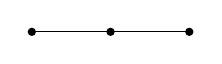
\begin{tikzpicture}
    \draw (0, 0) node [circ] {} -- (2, 0) node [circ] {} node [pos=0.5, circ] {};
  \end{tikzpicture}}
  \quad\quad
  \makecenter{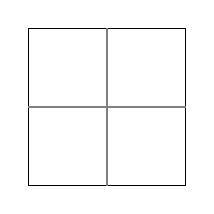
\begin{tikzpicture}
    \draw (0, 0) rectangle (2, 2);
    \draw [gray] (1, 0) -- (1, 2);
    \draw [gray] (0, 1) -- (2, 1);
  \end{tikzpicture}}
  \quad\quad
  \makecenter{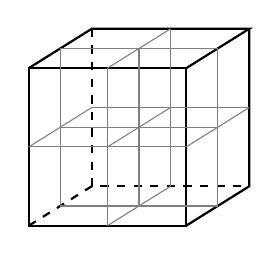
\begin{tikzpicture}
    \draw [thick] (0, 0) rectangle (2, -2);
    \draw [thick] (0, 0) -- (0.8, 0.5) -- (2.8, 0.5) -- (2, 0);
    \draw [thick] (2.8, 0.5) -- (2.8, -1.5) -- (2, -2);
    \draw [dashed, thick] (0.8, 0.5) -- (0.8, -1.5) -- (2.8, -1.5);
    \draw [dashed, thick] (0, -2) -- (0.8, -1.5);

    \draw [gray] (1, 0) -- (1, -2);
    \draw [gray] (0, -1) -- (2, -1);

    \draw [gray] (1.8, 0.5) -- (1.8, -1.5);
    \draw [gray] (0.8, -0.5) -- (2.8, -0.5);

    \draw [gray] (1, 0) -- (1.8, 0.5);
    \draw [gray] (1, -2) -- (1.8, -1.5);

    \draw [gray] (2, -1) -- (2.8, -0.5);
    \draw [gray] (0, -1) -- (0.8, -0.5);

    \draw [gray] (0.4, -0.75) -- (2.4, -0.75);

    \draw [gray] (1.4, 0.25) -- (1.4, -1.75);

    \draw [gray] (0.4, 0.25) -- (2.4, 0.25) -- (2.4, -1.75);
    \draw [gray] (0.4, 0.25) -- (0.4, -1.75) -- (2.4, -1.75);

    \draw [gray] (1, -1) -- (1.8, -0.5);
  \end{tikzpicture}}
\end{center}
Then since $C(L)$ contains $2^D$ disjoint copies of $C(L/2)$ (note that it is not exactly the union of them, since we are missing some boundary points), we know that
\[
  \vol(C(L)) \geq \sum_{i = 1}^{2^D} \vol(C(L/2)) = 2^D \vol(C(L/2)),
\]
Now in the case of an infinite dimensional vector space, $C(L)$ will contain \emph{infinitely many} copies of $C(L/2)$. So since $\vol(C(L/2))$ must be non-zero, as it is open, we know $\vol(C(L))$ must be infinite, and this is true for any $L$. Since any open set must contain some open hypercube, it follows that all open sets have infinite measure, and we are dead.

\begin{thm}
  There are no Lebesgue measures on an infinite dimensional inner product space.
\end{thm}

This means whenever we do path integrals, we need to understand that we are not actually doing an integral in the usual sense, but we are just using a shorthand for the limit of the discretized integral
\[
  \lim_{N \to \infty} \left(\frac{1}{2\pi \Delta t}\right)^{nN/2} \int \prod_{i = 1}^{N - 1} \d^n x_i\; \exp\left(- \frac{1}{2}\left(\frac{|x_{i + 1}- x_i|}{\Delta t}\right)^2 \Delta t\right).
\]
as a whole. In particular, we cannot expect the familiar properties of integrals to always hold for our path integrals.

If we just forget about this problem and start to do path integrals, then we would essentially be writing down nonsense. We can follow perfectly logical steps and prove things, but the output will still be nonsense. Then we would have to try to invent some new nonsense to make sense of the nonsense. This was, in fact, how renormalization was invented! (but as we will see, that is not what renormalization really is about)

Note that we showed that the measure $\D x$ doesn't exist, but what we really need wasn't $\D x$. What we really needed was
\[
  \int \D x e^{-S[x]}.
\]
This is no longer translation invariant, so it is conceivable that it exists. Indeed, in the case of a 1D quantum field theory, it does, and is known as the \term{Wiener measure}.

In higher dimensions, we are less certain. We know it doesn't exist for QED, and we believe it does not exist for the standard model. However, we believe that it does exist for Yang-Mills theory in four dimensions.

\subsubsection*{Non-commutativity in QM}
Now we know that the path integral measure doesn't exist, and this will solve our problem with non-commutativity. Indeed, as we analyze the discretization of the path integral, the fact that
\[
  [\hat{x}, \hat{p}] \not= 0
\]
will fall out naturally.

Again, consider a free theory, and pick times
\[
  T > t_+ > t > t_- > 0.
\]
We will consider
\begin{align*}
  \int \D x\; x(t) \dot{x}(t_-) e^{-S} &= \brak{y_1} e^{-H(T - t)} \hat{x} e^{-H(t - t_-)} \hat{p} e^{-H t_-} \bket{y_0},\\
  \int \D x\; x(t) \dot{x}(t_+) e^{-S} &= \brak{y_1} e^{-H(t - t_+)} \hat{p} e^{-H (t_+ - t)} \hat{x} e^{-Ht}\bket{y_0}.
\end{align*}
As we take the limit $t_{\pm} \to t$, the difference of the right hand sides becomes
\[
  \brak{y_1} e^{-H(t - t) }[\hat{x}, \hat{p}] e^{-H t}\bket{y_0} = \brak{y_1} e^{-HT} \bket{y_0} \not= 0.
\]
On the other hand, in the continuum path integral, the limit seems to give the same expression in both cases, and the difference vanishes, naively. The problem is that we \emph{need} to regularize. We cannot just bring two operators together in time and expect it to behave well. This is just like in perturbation theory, when we bring two events together in time, we have to worry that the propagators become singular.

Normally, we would have something like
\[
  x(t) \dot{x}(t_-) - x(t) \dot{x}(t_+) = x_t \left(\frac{x_{t_-} - x_{t_- - \Delta t}}{\Delta t}\right) - x_t \left(\frac{x_{t_+ + \Delta t} - x_{t_+}}{ \Delta t}\right).
\]
In the regularized integral, we can keep increasing $t_-$ and decreasing $t_+$, until we get to the point
\[
  x_t \left(\frac{x_t - x_{t - \Delta t}}{\Delta t}\right) - x_t \left(\frac{x_{t + \Delta t} - x_t}{ \Delta t}\right).
\]
Now that $t_{\pm}$ have hit $t$, we need to look carefully what happens to the individual heat kernels. In general, we stop taking the limit as soon as any part of the discretized derivative touches $x_t$. The part of the integral that depends on $x_t$ looks like
\[
  \int \d^n x_t\; K_{\Delta t}(x_{t + \Delta t}, x_t) x_t \left(\frac{x_t - x_{t - \Delta t}}{\Delta t} - \frac{x_{t + \Delta t} - x_t}{ \Delta t}\right) K_{\Delta t} (x_t, x_{t - \Delta t}).
\]
Using the fact that
\[
  K_{\Delta t}(x_t, x_{t - \Delta t}) \sim \exp\left(- \frac{(x_t - x_{t - \Delta t})^2}{2\Delta t}\right),
\]
we can write the integral as
\[
  \int \d^n x_t \; x_t \frac{\partial}{\partial x_t} \Big(K_{\Delta t}(x_{t + \Delta t}, x_t) K_{\Delta t}(x_t, x_{t - \Delta t})\Big),
\]
Now integrating by parts, we get that this is equal to
\[
  \int \d^n x_t\; K_{\Delta t} (x_{t + \Delta t}, x_t) K_{\Delta t} (x_t, x_{t - \Delta t}) = K_{2 \Delta t} (x_{t + \Delta t}, x_{t - \Delta t}).
\]
So we get the same as in the operator approach.

\subsection{Effective quantum field theory}
We now see what happens when we try to obtain effective field theories in 1 dimension. Suppose we have two real-valued fields $x, y: S^1 \to \R$. We pick the circle as our universe so that we won't have to worry about boundary conditions. We pick the action
\[
  S[x, y] = \int_{S^1} \left(\frac{1}{2} \dot{x}^2 + \frac{1}{2} \dot{y}^2 + \frac{1}{2} m^2 x^2 + \frac{1}{2}M^2 y^2 + \frac{\lambda}{4} x^2y^2 \right)\;\d t.
\]
As in the zero-dimensional case, we have Feynman rules
\begin{center}
  \makecenter{
  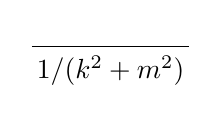
\begin{tikzpicture}
    \draw (0, 0) -- (2, 0) node [pos=0.5, below] {$1/(k^2 + m^2)$} node [pos=0.5, above] { };
  \end{tikzpicture}}\quad\quad
  \makecenter{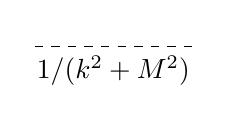
\begin{tikzpicture}
    \draw [dashed] (0, 0) -- (2, 0) node [pos=0.5, below] {$1/(k^2 + M^2)$} node [pos=0.5, above] { };
  \end{tikzpicture}}\quad\quad
  \makecenter{\begin{tikzpicture}[scale=0.707]
    \draw (0, 0) -- (2, 2);
    \draw [dashed] (0, 2) -- (2, 0);
    \node [circ] at (1, 1) {};
    \node [right] at (2, 1) {$-\lambda$};
  \end{tikzpicture}}
\end{center}
As in the case of zero-dimensional QFT, if we are only interested in the correlations involving $x(t)$, then we can integrate out the field $y(t)$ first. The effective potential can be written as
\[
  \int \D y\; \exp\left(-\frac{1}{2} \int_{S^1} y\left(-\frac{\d^2}{\d t^2} + M^2 + \frac{\lambda x^2}{2}\right) y \;\d t\right),
\]
where we integrated by parts to turn $\dot{y}^2$ to $y \ddot{y}$.

We start doing dubious things. Recall that we previously found that for a bilinear operator $M: \R^n \times \R^n \to \R$, we have
\[
  \int_{\R^n} \d^n x\; \exp\left(- \frac{1}{2} M(x, x)\right) = \frac{(2 \pi)^{n/2}}{\sqrt{\det{M}}}.
\]
Now, we can view our previous integral just as a Gaussian integral over the operator
\[
  (y, \tilde{y}) \mapsto \int_{S^1} y\left(-\frac{\d^2}{\d t^2} + M^2 + \frac{\lambda x^2}{2}\right) \tilde{y} \;\d t
\]
on the vector space of fields. Thus, (ignoring the factors of $(2\pi)^{n/2}$) we can formally write the integral as
\[
  \det \left(-\frac{\d^2}{\d t^2} + M^2 + \frac{\lambda x^2}{2}\right)^{-1/2}.
\]
$S_{\mathrm{eff}}[x]$ thus looks like
\[
  S_{\mathrm{eff}}[x] = \int_{S^1} \frac{1}{2}(\dot{x}^2 + m^2 x^2) \;\d t + \frac{1}{2} \log \det \left(-\frac{\d^2}{\d t^2} + M^2 + \frac{\lambda x^2}{2}\right)
\]
We now continue with our formal manipulations. Noting that $\log \det = \tr \log$, since $\det$ is the product of eigenvalues and $\tr$ is the sum of them, and factoring
\[
  -\frac{\d^2}{\d t^2} + M^2 + \frac{\lambda x^2}{2} = \left(-\frac{\d^2}{\d t^2} + M^2\right)\left(1 - \lambda \left(-\frac{\d^2}{\d t^2} + M^2\right)^{-1} \frac{x^2}{2}\right),
\]
we can write the last term in the effective potential as
\[
 \frac{1}{2} \tr \log \left(-\frac{\d^2}{\d t^2} + M^2\right) + \frac{1}{2} \tr \log \left(1 - \lambda \left(\frac{\d^2}{\d t^2} - M^2\right)^{-1} \frac{x^2}{2}\right)
\]
The first term is field independent, so we might as well drop it. We now look carefully at the second term. The next dodgy step to take is to realize we know what the inverse of the differential operator
\[
  \frac{\d^2}{\d t^2} - M^2
\]
is. It is just the Green's function! In other words, it is given by the function $G(t, t')$ such that
\[
  \left(\frac{\d^2}{\d t^2} - M^2 \right) G(t, t') = \delta(t - t').
\]
The solution to this is given by
\[
  G(t, t') = \frac{1}{2M} \sum_{n \in \Z} \exp\left(-M |t - t' + \beta k|\right),
\]
with
\[
  \beta = \frac{1}{T}.
\]
Using this, we claim that we can expand the last term in the effective potential as
\begin{multline*}
  \tr \log \left(1 - \lambda G(t, t') \frac{x^2}{2}\right) \\
  = - \frac{\lambda}{2} \int_{S_1}G(t, t) x^2(t) \;\d t - \frac{\lambda^2}{8} \int_{S^1 \times S^1} \d t\; \d t' G(t', t) x^2(t) G(t, t') x^2(t') \cdots
\end{multline*}
We can vaguely imagine a justification of this expansion as follows --- we expand the logarithm in Taylor series. The first term comes from $\frac{\lambda}{2}G(t, t) x^2(t)$, where the trace operator means we put $t = t'$. The second term comes from the square of $\frac{\lambda}{2} G(t, t') x^2$, and taking the trace of the square means we integrate over things going from $t$ to $t'$, then back to $t$, etc.

Now we see that these terms are \emph{non-local}! It involves integrating over many different points in $S^1$. In fact, we should have expected this non-locality from the corresponding Feynman diagrams. The first term corresponds to
\begin{center}
  \begin{tikzpicture}
    \node [circ, mblue] at (0, 0) {};
    \node [above] at (0, 0) {$x(t)$};
    \node [circ, mblue] at (0, -2) {};
    \node [below] at (0, -2) {$x(t)$};
    \draw (0, 0) -- (0, -2);

    \node [circ] at (0, -1) {};

    \draw [dashed] (0.4, -1) ellipse (0.4 and 0.25);
  \end{tikzpicture}
\end{center}
Here $G(t, t)$ corresponds to the $y$ field.

The second diagram we have looks like this:
\begin{center}
  \begin{tikzpicture}[eqpic]
    \draw (-0.2, 0) node [circ, mblue] {} node [above] {$x(t)$} -- +(0.2, -1) node [circ] {} -- +(0, -2) node [circ, mblue] {} node [below] {$x(t)$};
    \draw (1, 0) node [circ, mblue] {} node [above] {$x(t')$} -- +(-0.2, -1) node [circ] {} -- +(0, -2) node [circ, mblue] {} node [below] {$x(t')$};
    \draw [dashed] (0.4, -1) ellipse (0.4 and 0.25);
  \end{tikzpicture}
\end{center}
We see that the first diagram is local, as there is just one vertex at time $t$. But in the second diagram, we use the propagators to allow the $x$ at time $t$ to talk to $x$ at time $t'$. This is non-local!

Non-locality is generic. Whenever we integrate out our fields, we get non-local terms. But non-locality is terrible in physics. It means that the equations of motion we get, even in the classical limit, are going to be integral differential equations, not just normal differential equations. For a particle to figure out what it should do here, it needs to know what is happening in the far side of the universe!

To make progress, we note that if $M$ is very large, then we would expect $G(t, t')$ could be highly suppressed for $t \not= t'$. So we can try to expand around $t = t'$. Recall that the second term is given by
\[
  \int \d t\; \d t' G(t, t')^2 x^2(t) x'(t^2)
\]
We can write out $x'(t^2)$ as
\[
  x'(t^2) = x^2 (t) + 2x(t) \dot{x}(t) (t' - t) + \left(\dot{x}^2(t) + \frac{1}{2} x(t) \dot{x}(t)\right) (t - t')^2 + \cdots.
\]
Using the fact that $G(t, t')$ depends on $t'$ only through $M(t' - t)$, by dimensional analysis, we get an expansion that looks like
\[
  \frac{1}{M^2} \int \d t\; \frac{\alpha}{M} x^4(t) + \frac{\beta}{M^3} \left(x^2 \dot{x}^2 + \frac{1}{2} x^2 \ddot{x}\right) + \frac{\gamma}{M^5} (\text{4-derivative terms}) + \cdots
\]
Here $\alpha, \beta, \gamma$ are dimensionless quantities.

Thus, we know that every extra derivative is accompanied by a further power of $\frac{1}{M}$. Thus, provided $x(t)$ is slowly varying on scales of order $\frac{1}{M}$, we may hope to truncate the series.

Thus, at energies $E \ll M$, our theory looks approximately local. So as long as we only use our low-energy approximation to answer low-energy questions, we are fine. However, if we try to take our low-energy theory and try to extrapolate it to higher and higher energies, up to $E \sim M$, it is going to be nonsense. In particular, it becomes non-unitary, and probability is not preserved.

This makes sense. By truncating the series at the first term, we are ignoring all the higher interactions governed by the $y$ fields. By ignoring them, we are ignoring some events that have non-zero probability of happening, and thus we would expect probability not to be conserved.

There are two famous examples of this. The first is weak interactions. At very low energies, weak interactions are responsible for $\beta$-decay. The effective action contains a quartic interaction
\[
  \int \d^4 x\; \bar\psi_e n \nu_e p \; G_{\mathrm{weak}}.
\]
This coupling constant $G_{\mathrm{weak}}$ has mass dimensional $-1$. At low energies, this is a perfectly well description of beta decay. However, this is suspicious. The fact that we have a coupling constant with negative mass dimension suggests this came from integrating some fields out.

At high energies, we find that this \emph{4-Fermi theory} becomes non-unitary, and $G_{\mathrm{weak}}$ is revealed as an approximation to a $W$-boson propagator. Instead of an interaction that looks like this:
\begin{center}
  \begin{tikzpicture}
    \draw (0, 0) -- (2, 2);
    \draw (0, 2) -- (2, 0);
    \node [circ] at (1, 1) {};
  \end{tikzpicture}
\end{center}
what we really have is
\begin{center}
  \begin{tikzpicture}
    \draw (0, 0) -- (0.75, 1) -- (0, 2);

    \draw [decorate, decoration={snake}](0.75, 1) -- (2.25, 1) node [pos=0.5, above=0.3em] {$W$};
    \draw (3, 2) -- (2.25, 1) -- (3, 0);
    \node [circ] at (0.75, 1) {};
    \node [circ] at (2.25, 1) {};
  \end{tikzpicture}
\end{center}
There are many other theories we can write down that has negative mass dimension, the most famous one being general relativity.

\subsection{Quantum gravity in one dimension}
In quantum gravity, we also include a (path) integral over all metrics on our spacetime, up to diffeomorphism invariance. We also sum over all possible topologies of $M$. In $d = 1$ (and $d = 2$ for string theory), we can just do this.

In $d = 1$, a metric $g$ only has one component $g_{tt}(t) = e(t)$. There is no curvature, and the only diffeomorphism invariant of this metric is the total length
\[
  T = \oint e(t) \;\d t.
\]
So the instruction to integrate over all metrics modulo diffeomorphism is just the instruction to integrate over all possible lengths of the worldline $T \in (0, \infty)$, which is easy. Let's look at that.

The path integral is given by
\[
  \int_T \d T \;\int_{C_{[0, T]} [y, x]} \D x\; e^{-S[x]}.
\]
where as usual
\[
  S[x] = \frac{1}{2} \int_0^T \dot{x}^2 \;\d t.
\]
Just for fun, we will include a ``cosmological constant'' term into our action, so that we instead have
\[
  S[x] = \frac{1}{2} \int_0^T \dot{x}^2 + \frac{m^2}{2}\;\d t.
\]
The reason for this will be revealed soon.

We can think of the path integral as the heat kernel, so we can write it as
\begin{align*}
  \int_0^\infty\; \d T\; \brak{y} e^{-HT} \bket{x} &= \int_0^\infty \d T\; \frac{\d^n p\; \d^n q}{ (2\pi)^n} \braket{y}{q} \brak{q} e^{-HT}\bket{p} \braket{p}{x}\\
  &= \int_0^\infty \d T\; \frac{\d^n p\; \d ^n q}{(2\pi)^n} e^{ip\cdot x - i q \cdot y} e^{-T(p^2 + m^2)/2} \delta^n(p - q)\\
  &= \int_0^\infty \d T\; \frac{\d^n p}{(2\pi)^n} e^{ip\cdot (x - y)} e^{-T(p^2 + m^2)/2}\\
  &= 2 \int \frac{\d^n p}{(2\pi)^n} \frac{e^{ip\cdot (x - y)}}{p^2 + m^2}\\
  &= 2 D(x, y),
\end{align*}
where $D(x, y)$ is the propagator for a scalar field on the \emph{target space} $\R^n$ with action
\[
  S[\Phi] = \int \d^n x \; \frac{1}{2} (\partial \Phi)^2 + \frac{m^2}{2} \Phi^2.
\]
So a $1$-dimensional quantum gravity theory with values in $\R^n$ is equivalent to (or at least has deep connections to) a scalar field theory on $\R^n$.

How about interactions? So far, we have been taking rather unexciting 1-dimensional manifolds as our universe, and there are only two possible choices. If we allow singularities in our manifolds, then we would allow \emph{graphs} instead of just a line and a circle. Quantum gravity then says we should not only integrate over all possible lengths, but also all possible graphs.

For example, to compute correlation functions such as $\bra \Phi(x_1) \cdots \Phi(x_n)\ket$ in $\Phi^4$ theory on $\R^n$, say, we consider all $4$-valent with $n$ external legs with one endpoint at each of the $x_i$, and then we proceed just as in quantum gravity.

For example, we get a contribution to $\bra \Phi(x) \Phi(y)\ket$ from the graph
\begin{center}
  \begin{tikzpicture}
    \draw (0, 0) node [circ] {} node [left] {$x$} -- (2, 0) node [circ] {} node [right] {$x$};

    \node [circ] at (1, 0) {};
    \draw (1, 0.4) ellipse (0.2 and 0.4);
  \end{tikzpicture}
\end{center}
The contribution to the quantum gravity expression is
\begin{multline*}
  \int\limits_{\mathclap{z \in \R^n}}\d^n z \int\limits_{\mathclap{[0, \infty)^3}} \d T_1\, \d T_2\, \d T_3\, \int\limits_{\mathclap{\mathcal{C}_{T_1}[z, x]}} \D x\, e^{-S_{T_1}[x]} \int\limits_{\mathclap{C_{T_2}[z, z]}} \D x\, e^{-S_{T_2}[x]} \int\limits_{\mathclap{C_{T_3}[y, z]}} \D x\, e^{-S_{T_3}[x]},
\end{multline*}
where
\[
  S_T[x] = \frac{1}{2} \int_0^T x^2 \;\d t + \frac{m^2}{2}\int_0^T \d t.
\]
We should think of the second term as the ``cosmological constant'', while the 1D integrals over $T_i$'s are the ``1d quantum gravity'' part of the path integral (also known as the \term{Schwinger parameters} for the graph).

We can write this as
\begin{align*}
  &\hphantom{{}={}} \int \d^n z \; \d T_1 \;\d T_2 \;\d T_3\; \brak{z} e^{-HT_1} \bket{x} \brak{z}e^{-HT_2} \bket{z} \brak{y} e^{-H T_3} \bket{z}.\\
  \intertext{Inserting a complete set of eigenstates between the position states and the time evolution operators, we get}
  &= \int \frac{\d^n p\; \d^n \ell\;\d^n q}{(2\pi)^{3n}} \frac{e^{ip\cdot(x - z)}}{p^2 + m^2} \frac{e^{iq\cdot(y - z)}}{q^2 + m^2} \frac{e^{i\ell\cdot(z - z)}}{\ell^2 + m^2}\\
  &= \int \frac{\d^n p\; \d^n \ell}{(2\pi)^{2n}} \frac{e^{ip\cdot (x - y)}}{(p^2 + m^2)^2} \frac{1}{\ell^2 + m^2}.
\end{align*}
This is exactly what we would have expected if we viewed the above diagram as a Feynman diagram:
\begin{center}
  \begin{tikzpicture}
    \draw (0, 0) node [circ] {} node [left] {$x$} -- (2, 0) node [circ] {} node [right] {$y$};

    \node at (0.5, 0) [below] {$p$};
    \node at (1.5, 0) [below] {$p$};

    \node [circ] at (1, 0) {};
    \draw (1, 0.4) ellipse (0.2 and 0.4);
    \node at (1.2, 0.4) [right] {$\ell$};
  \end{tikzpicture}
\end{center}
This is the \term{worldline perspective} to QFT, and it was indeed Feynman's original approach to doing QFT.

\section{Symmetries of the path integral}
From now on, we will work with quantum field theory in general, and impose no restrictions on the dimension of our universe. The first subject to study is the notion of symmetries.

In classical field theory, symmetries played a huge role. In particular, Noether's theorem relates symmetries to conservation laws. For simplicity, we will work with the case of a flat space.

Suppose we had a variation
\[
  \delta \phi = \varepsilon f(\phi, \partial \phi)
\]
of the field. The most common case is when $f(\phi, \partial \phi)$ depends on $\phi$ only locally, in which case we can think of the transformation as being generated by the vector
\[
  V_f = \int_M \d^d x \; f(\phi, \partial \phi) \frac{\delta}{\delta \phi(x)}
\]
acting on the space of fields. If the function $S[\phi]$ is invariant under $V_f$ when $\varepsilon$ is constant, then for general $\varepsilon(x)$, we must have
\[
  \delta S = \int \d^d x\; j^\mu(x) \partial_\mu \varepsilon.
\] % see notes for more general thing
for some field-dependent current $j_\mu(x)$. If we choose $\varepsilon(x)$ to have compact support, then we can write
\[
  \delta S = - \int \d^d x\; (\partial^\mu j_\mu) \varepsilon(x).
\]
On \emph{solutions} of the field equation, we know the action is stationary under arbitrary variations. So $\delta S = 0$. Since $\varepsilon(x)$ was arbitrary, we must have
\[
  \partial^\mu j_\mu = 0.
\]
So we know that $j_\mu$ is a \term{conserved current}.

Given any such conserved current, we can define the \term{charge} $Q[N]$ associated to an (oriented) co-dimension $1$ hypersurface $N$ as
\[
  Q[N] = \int_N n^\mu j_\mu\; \d^{d - 1}x,
\]
where $n^\mu$ is the normal vector to $N$. Usually, $N$ is a time slice, and the normal points in the future direction.

Now if $N_0$ and $N_1$ are two such hypersurfaces bounding a region $M' \subseteq M$, then by Stokes' theorem, we have
\[
  Q[N_0] - Q[N_1] = \left(\int_{N_0} - \int_{N_1}\right) n^\mu j_\mu \;\d^{n - 1}x = \int_{M'} (\partial^\mu j_\mu)\;\d^n x = 0.
\]
So we find
\[
  Q[N_0] = Q[N_1].
\]
This is the conservation of charge! This is the classical picture.

\subsection{Ward identities}
The derivation of Noether's theorem used the classical equation of motion. But in a quantum theory, the equation of motion no longer holds. We must re-examine what happens in the quantum theory.

Suppose a transformation $\phi \mapsto \phi'$ of the fields has the property that
\[
  \D \phi\; e^{-S[\phi]} = \D \phi'\; e^{-S[\phi']}.
\]
In theory, the whole expression $\D \phi\; e^{-S[\phi]}$ is what is important in the quantum theory. In practice, we often look for symmetries where $\D \phi$ and $e^{-S[\phi]}$ are separately conserved. In fact, what we will do is that we look for a symmetry that preserves $S[\phi]$, and then try to find a regularization of $\D \phi$ that is manifestly invariant under the symmetry.

Often, it is not the case that the obvious choice of regularization of $\D \phi$ is manifestly invariant under the symmetry. For example, we might have a $\phi$ that is rotationally invariant. However, if we regularize the path integral measure by picking a lattice and sampling $\phi$ on different points, it is rarely the case that this lattice is rotationally invariant.

In general, there are two possibilities:
\begin{enumerate}
  \item The symmetry could be restored in the limit. This typically means there exists a regularized path integral measure manifestly invariant under this symmetry, but we just didn't use it. For example, rotational invariance is not manifestly present in lattice regularization, but it is when we do the cut-off regularization.
  \item It could be that the symmetry is not restored. It is said to be \emph{anomalous}\index{anomalous symmetry}, ie. broken in the quantum theory. In this case, there can be no invariant path integral measure. An example is scale invariance in QED, if the mass of the electron is $0$.
\end{enumerate}
Sometimes, it can be hard to tell. For now, let's just assume we are in a situation where $\D \phi = \D \phi'$ when $\varepsilon$ is constant. Then for any $\varepsilon(x)$, we clearly have
\[
  \mathcal{Z} = \int \D \phi\; e^{-S [\phi]} = \int \D \phi' e^{-S[\phi']},
\]
since this is just renaming of variables. But using the fact that the measure is invariant when $\varepsilon$ is constant, we can can expand the right-hand integral in $\varepsilon$, and again argue that it must be of the form
\[
  \int \D \phi'\; e^{-S[\phi']} = \int \D \phi\; e^{-S[\phi]} \left(1 - \int_M j_\mu \partial^\mu \varepsilon\; \d^n x\right).
\]
in first order in $\varepsilon$. Note that in general, $j_\mu$ can receive contributions from $S[\phi]$ and $\D \phi$. So we know
\[
  \int \D \phi e^{-S[\phi]} \int_M j^\mu \partial_\mu \varepsilon \;\d^d x = 0.
\]
Integrating by parts, and using the definition of the expectation, we can write this as
\[
  -\int_M \varepsilon \partial^\mu \bra j_\mu (x)\ket\; \d^n x,
\]
for any $\varepsilon$ with compact support. Note that we dropped a normalization factor of $\mathcal{Z}$ in the definition of $\bra j_\mu(x)\ket$, because $\mathcal{Z}$ times zero is still zero. So we know that $\bra j_\mu (x)\ket$ is a conserved current, just as we had classically.

One of the main uses of symmetries is to constrain correlation functions.

Suppose we have an operator $\mathcal{O}$ that depends only on $\phi$, and not its derivatives. Then under a transformation $\phi \mapsto \phi'$, our operator transforms as
\[
  \mathcal{O}(\phi) \mapsto \mathcal{O}(\phi'),
\]
Now we further suppose this transformation is a symmetry. By definition, we can write
\[
  \bra \mathcal{O}_1(x_1) \cdots \mathcal{O}_n(x_n)\ket = \frac{1}{\mathcal{Z}} \int \D \phi e^{-S[\phi]} \mathcal{O}_1(\phi(x_1)) \cdots \mathcal{O}_n(\phi(x_n)).
\]
Trivially, by renaming of variables, this is equal to
\[
  \frac{1}{\mathcal{Z}} \int \D \phi' e^{-S[\phi']} \mathcal{O}_1(\phi'(x_1)) \cdots \mathcal{O}_n(\phi'(x_n)).
\]
Using the invariance of the measure, this is equal to
\[
  \frac{1}{\mathcal{Z}} \int \D \phi\;e^{-S[\phi]} \mathcal{O}_1(\phi'(x_1) \cdots \mathcal{O}_n (\phi'(x_n)).
\]
Consequently, we find
\[
  \bra \mathcal{O}_1(\phi(x_n)) \cdots \mathcal{O}_n(\phi(x_n))\ket = \bra \mathcal{O}_1(\phi'(x_n)) \cdots \mathcal{O}_n(\phi'(x_n))\ket.
\]
So the correlation function of the original and transformed operators are the agree \emph{in the same theory}.

\begin{eg}
  Suppose we have a transformation $\phi \mapsto \phi' = e^{i\alpha}\phi$ for some $\alpha \in \R/2\pi \Z$, for some complex field $\phi$. Consequently, the conjugate field transforms as
  \[
    \bar\phi \mapsto \bar\phi' =e^{-i\alpha} \bar\phi.
  \]
  Suppose this transformation preserves the action and measure. For example, the measure will be preserved if we integrate over the same number of $\phi$ and $\bar\phi$ modes. Consider the operators
  \[
    \mathcal{O}_i (\phi, \bar\phi) = \bar\phi^{s_i} \bar\phi(x)^{r_i}.
  \]
  Then we have
  \[
    \mathcal{O}_i(\phi, \bar\phi) \mapsto \mathcal{O}_i (\phi', \bar\phi') = e^{-\alpha (r_i - s_i)} \mathcal{O}_i(\phi, \bar\phi).
  \]
  Thus we know that
  \[
    \left\bra \prod_{i = 1}^m \mathcal{O}_i(x_i)\right\ket = \exp\left(i \alpha \sum_{i = 1}^m (r_i - s_i)\right) \left\bra \prod_{i = 1}^m \mathcal{O}_i(x_i)\right\ket.
  \]
  Consequently, since this is true for all $\alpha$, we know that the correlation function
  \[
    \mathcal{O}_i(\phi, \bar\phi) \mapsto \mathcal{O}_i (\phi', \bar\phi')
  \]
  must vanish, unless
  \[
    \sum_{i = 1}^m r_i = \sum_{i = 1}^m s_i.
  \]
  So we need the same number of $\phi$ and $\bar\phi$ insertions in total.

  We could also have obtained this result from Feynman graphs. We simply have to note that each propagator join up a $\phi$ and $\bar\phi$ together. So if we don't have equal number of $\phi$ and $\bar\phi$, then we can't draw any Feynman diagrams at all! So the correlator must vanish.
\end{eg}

\begin{eg}
  Consider $(M, g) = (\R^4, \delta)$, and consider spacial translation $x \mapsto x' = x - a$ for a constant vector $a$. A scalar field $\phi$ transforms as
  \[
    \phi(x) \mapsto \phi'(x) = \phi(x - a).
  \]
  In most cases, this is a symmetry. So the scalar operators transform as $\mathcal{O}(\phi(x)) \mapsto \mathcal{O}(\phi(x - a))$. In shorthand, we write $\mathcal{O}(x) \mapsto \mathcal{O}(x - a)$.

  Thus, we find that.
  \[
    \bra \mathcal{O}_1(x_1) \cdots \mathcal{O}_n(x_n)\ket = \bra \mathcal{O}_1(x_1 - a) \cdots \mathcal{O}_n(x_n - a)\ket.
  \]
  Hence, the correlation function must depend only on the separation $x_{ij} = x_i - x_j$. Similarly, if the action and measure are rotationally or Lorentz invariant, then under a transformation $L$, we find
  \[
    \bra \mathcal{O}(x_1) \cdots \mathcal{O}_n(x_n)\ket = \bra \mathcal{O}_1(L x_1) \cdots \mathcal{O}_n (L x_n)\ket.
  \]
  So the correlation only depends on the Lorentz invariant separations $x_{ij}^2$.
\end{eg}

\subsubsection*{Ward identity for correlators}
So far, we have just been talking about properties of symmetries. We haven't used the induced conserved current at all. So let's try to do some Noether's theorem-like manipulations.

Suppose we have an infinitesimal transformation, with $\phi \mapsto \phi + \varepsilon \delta \phi$ that is a symmetry when $\varepsilon$ is constant. Then for general $\varepsilon(x)$ we have
\begin{align*}
  &\hphantom{={}} \int \D \phi\; e^{-S[\phi]} \mathcal{O}_1(\phi(x_1) \cdots \mathcal{O}_n(\phi(x_n)) \\
  &= \int \D \phi'\; e^{-S[\phi']} \mathcal{O}_1(\phi'(x_1) \cdots \mathcal{O}_n(\phi'(x_n))\\
  &= \int \D \phi e^{-S[\phi]} \left(1 - \int j^\mu (x) \partial_\mu \varepsilon(x) \;\d x\right)\left(\mathcal{O}_1(\phi(x_1)) \cdots \mathcal{O}_n(\phi(x_n))\vphantom{ + \sum_{i = 1}^n \varepsilon(x_i) \delta \mathcal{O}(x_i) \prod_{j \not= i} \mathcal{O}_j(x_j)}\right.\\
  &\hphantom{= \int \D \phi e^{-S[\phi]} \left(1 - \int j^\mu (x) \partial_\mu \varepsilon(x) \;\d x\right)}\left.+ \sum_{i = 1}^n \varepsilon(x_i) \delta \mathcal{O}_i(x_i) \prod_{j \not= i} \mathcal{O}_j(x_j)\right),
\end{align*}
where
\[
  \delta \mathcal{O}(x_i) = \frac{\partial \mathcal{O}}{\partial \phi} \delta \phi.
\]
Again, the zeroth order piece of the correlation function cancels, and to lowest non-trivial order, we find that we must have
\[
   \int \partial^\mu \varepsilon(x) \left\bra j_\mu(x) \prod_{i = 1}^n \mathcal{O}_i(x_i)\right\ket\;\d^d x = \sum_{i = 1}^m \varepsilon(x_i) \left\bra \delta \mathcal{O}_i(x_i) \prod_{j \not= i} \mathcal{O}_j(x_j)\right\ket.
\]
We want to get rid of the $\varepsilon$ dependence, but we can't just strip it off by integrating by parts, as in the first term, it is integrated over all space, while on the right, it is evaluated at specific points.

What we need is a little trick. We integrate the left hand side by parts, and write the right as an integral of $\delta$-functions:
\begin{multline*}
  \int \varepsilon(x) \partial^\mu \left\bra j_\mu(x) \prod_{i = 1}^n \mathcal{O}_i(x_i)\right\ket\;\d^d x \\
  = - \sum_{i = 1}^m \int \varepsilon(x) \delta^d(x - x_i) \left\bra \delta \mathcal{O}_i(x_i) \prod_{j \not= i} \mathcal{O}_j(x_j)\right\ket \;\d^d x.
\end{multline*}
Since this holds for arbitrary $\varepsilon(x)$ (with compact support), we must have
\[
  \partial^\mu \left\bra j_\mu (x) \prod \mathcal{O}_i(x_i)\right\ket = -\sum_{i = 1}^n \delta^d(x - x_i)\left\bra \delta \mathcal{O}_i(x_i) \prod_{j \not= i} \mathcal{O}_j(x_j)\right\ket.
\]
This is the \term{Ward identity} for correlation functions. It says that the vector field
\[
  f_\mu (x, x_i) = \left\bra j_\mu (x) \prod_i \mathcal{O}_i x_i\right\ket
\]
is divergence free except at the insertions $x_i$.

To understand this, suppose $M$ is compact without boundary, and integrate the Ward identity over all $M$ (so that we don't worry about boundary terms). Then integrating over all of space, we find that
\[
  0 = \int_M \partial^\mu f_\mu(x, x_i)\;\d^d x = -\sum_{i = 1}^n \left\bra \delta \mathcal{O}_i(x_i) \prod_{j \not= i} \mathcal{O}_j(x_j)\right\ket = \delta \left\bra \prod_{i = 1}^n \mathcal{O}_i(x_i)\right\ket,
\]
where we get the first equality because by Stokes' theorem, the integral of \emph{any} divergence over a compact surface without boundary vanishes.

In other words, what we have is the correlation function must be invariant under the transformation. This is just the infinitesimal version of what we've seen already.

That was nothing new, but suppose $M' \subseteq M$ is a region with boundary $N_1 - N_0$, and let % picture!
\[
  I = \{i \in \{1, \cdots, n\}: x_i \in M'\}.
\]
Now integrating over $M'$ gives
\begin{align*}
  \int_{M'} \partial^\mu \left\bra j_\mu (x) \prod_{i = 1}^n \mathcal{O}_i(x_i)\right\ket &= \int_{N_1 - N_0} n^\mu\left\bra j_\mu (x) \prod_{i = 1}^n \mathcal{O}_i(x_i)\right\ket\;\d^{d - 1}x\\
  &= \left\bra Q[N_1] \prod_{i = 1}^n \mathcal{O}_i(x_i)\right\ket - \left\bra Q[N_0] \prod_{i = 1}^n \mathcal{O}_i(x_i)\right\ket
\end{align*}
Thus, by the Ward identity, we find
\[
  \left\bra Q[N_1] \prod_{i = 1}^n \mathcal{O}_i(x_i)\right\ket - \left\bra Q[N_0] \prod_{i = 1}^n \mathcal{O}_i(x_i)\right\ket = - \sum_{i \in I} \left\bra \delta \mathcal{O}_i(x_i) \prod_{j \not= i}^m \mathcal{O}_j(x_j)\right\ket.
\]
In particular, if $M'$ contains only one point, say $x_1$, and we choose the region to be infinitesimally thin, then in the canonical picture, we have
\[
  \brak{\Omega}\mathcal{T} [\hat{Q}, \hat{\mathcal{O}}_1(x_1)] \prod_{j = 2}^m \hat{\mathcal{O}}_j (x_j)\bket{\Omega} = - \brak{\Omega} \mathcal{T} \left\{\delta \hat{\mathcal{O}}_1 \prod_{j = 2}^n \hat{\mathcal{O}}_j(x_j)\right\}\bket{\Omega},
\]
where $\bket{\Omega}$ is some (vacuum) state. So in the canonical picture, we find that
\[
  \delta \hat{\mathcal{O}} = [\hat{Q}, \hat{\mathcal{O}}]. % sign?
\]
So we see that the change of $\hat{\mathcal{O}}$ under some transformation is given by the commutator with the charge operator.

\subsection{The Ward--Takahashi identity}
We focus on an important example of this. The QED action
\[
  S[A, \psi] = \int \frac{1}{4} F_{\mu\nu}F^{\mu\nu} + i \bar\psi \D \psi + m \bar\psi \psi
\]
is invariant under the global transformations
\[
  \psi (x) \mapsto e^{i\alpha} \psi(x),\quad A_\mu(x) \mapsto A_\mu(x)
\]
for $\alpha \in \R/2\pi \Z$. The path integral measure is also invariant under this transformation provided we integrate over equal numbers of $\psi$ and $\bar\psi$ modes in the regularization.

To obtain the Ward identity, we do the normal things --- we let $\alpha$ depend on position. So the transformations become
\[
  \psi (x) \mapsto e^{i\alpha (x)} \psi(x),\quad A_\mu(x) \mapsto A_\mu(x).
\]
Note that this is \emph{not} the gauge transformation, as we don't change the photon field.

Under this transformation, the classical action is no longer invariant, and we obtain
\[
  \delta S = \int j^\mu \partial_\mu \alpha \;\d^4 x,
\]
where
\[
  j^\mu (x) = \bar\psi (x) \gamma^\mu \psi(x).
\]
is just the current. This leads to a Ward identity
\[
  \partial^\mu \bra j_\mu(x) \psi(x_1) \bar\psi(x_2)\ket = - \delta^4(x - x_1) \bra \psi(x_1) \bar\psi(x_2)\ket + \delta^4(x - x_2) \bra \psi(x_1) \bar\psi(x_2)\ket,
\]
noting that the infinitesimal change in $\psi$ is just (proportional to) $\psi$ itself. As always, we found that when we computed the insertion of the current, it is divergence free except in at the insertion points $x_1$ and $x_2$.

Let's look at this in momentum space, which is how it is traditionally done. We consider the Fourier transform
\[
  \int \d^4 x_1 \; \d^4 x_2\; e^{ik_1 \cdot x_1} e^{-ik_2 \cdot x_2} \bra \psi(x_1) \bar\psi(x_2)\ket.
\]
But since the system is translation invariant, the correlation $\bra \psi(x_1) \bar\psi(x_2) \ket$ is only dependent on the separation between $x_1$ and $x_2$. So we can write this as
\[
  \int \d^4 y \;\d^4 x_2 e^{i(k_1 - k_2) \cdot x_2} e^{ik_1 \cdot y} \bra \psi(y) \bar\psi(0)\ket,
\]
where $y = x_1 - x_2$. We write the result as
\[
  \delta^4(k_1 - k_2) S(k_1),
\]
where
\[
  S(k) = \int \d^4 y\; e^{ik\cdot y} \bra \psi(y) \bar\psi(0)\ket
\]
is the \term{$2$-point function} of the electron field in momentum space. This definition is an exact object, but if we wanted to compute this in perturbation theory, we can draw the diagram
\[\arraycolsep=0.25em\def\arraystretch{2.2}
  \begin{array}{ccccc} % fix
  S(k) & \sim &
  \begin{tikzpicture}[eqpic]

    \draw [fill, white] (0.7, 0.3) rectangle (1.3, -0.3);
    \draw (0, 0) node [circ] {} node [above] {$\bar\psi$} -- (2, 0) node [circ] {} node [above] {$\psi$};
  \end{tikzpicture}
  &+&
  \begin{tikzpicture}[eqpic]
    \draw (0, 0) node [circ] {} node [above] {$\bar\psi$} -- (2, 0) node [circ] {} node [above] {$\psi$};

    \draw [fill] (0.7, 0.3) rectangle (1.3, -0.3);
  \end{tikzpicture}\\
  & & \displaystyle\frac{1}{i \slashed{k} + m} &+& \text{quantum corrections}.
\end{array}
\]
Here we are lazy and use a black box to denote all quantum corrections. If we are less lazy, we can write this as
\[
  \begin{tikzpicture}[eqpic]
    \draw (0, 0) node [circ] {} node [above] {$\bar\psi$} -- (2, 0) node [circ] {} node [above] {$\psi$};

    \draw [fill] (0.7, 0.3) rectangle (1.3, -0.3);
  \end{tikzpicture}
  =
  \begin{tikzpicture}[eqpic]
    \draw (0, 0) node [circ] {} node [above] {$\bar\psi$} -- (2, 0) node [circ] {} node [above] {$\psi$};

    \draw [fill=white] (1, 0) circle [radius=0.3] node {IPI};
  \end{tikzpicture}
  +
  \begin{tikzpicture}[eqpic]
    \draw (0, 0) node [circ] {} node [above] {$\bar\psi$} -- (3, 0) node [circ] {} node [above] {$\psi$};

    \draw [fill=white] (1, 0) circle [radius=0.3] node {IPI};
    \draw [fill=white] (2, 0) circle [radius=0.3] node {IPI};
  \end{tikzpicture}
  + \cdots
\]
where IPI is the sum of all \term{one-particle irreducible graphs}, ie. graphs connected graphs that cannot be disconnected by any single internal line.

For example, the following are one-particle irreducible graphs:
\begin{center}
  \begin{tikzpicture}
    \draw [white, decorate, decoration={snake}] (0.8, 0) arc(180:360:0.7) node [pos=0.5, above=0.5em] {$\gamma$};
    \draw (0, 0) node [circ] {} node [above] {$\bar\psi$} -- (3, 0) node [circ] {} node [above] {$\psi$};
    \draw [decorate, decoration={snake}] (0.8, 0) arc(180:0:0.7) node [pos=0.5, above=0.5em] {$\gamma$};
  \end{tikzpicture}
  \begin{tikzpicture}
    \draw (0, 0) node [circ] {} node [above] {$\bar\psi$} -- (3, 0) node [circ] {} node [above] {$\psi$};
    \draw [decorate, decoration={snake}] (0.5, 0) arc(180:0:0.7);
    \draw [decorate, decoration={snake}] (1.2, 0) arc(180:360:0.7);
  \end{tikzpicture}
\end{center}
while the following is not:
\begin{center}
  \begin{tikzpicture}
    \draw (0, 0) node [circ] {} node [above] {$\bar\psi$} -- (4.7, 0) node [circ] {} node [above] {$\psi$};
    \draw [decorate, decoration={snake}] (0.5, 0) arc(180:0:0.7);
    \draw [decorate, decoration={snake}] (2.8, 0) arc(180:0:0.7);
  \end{tikzpicture}
\end{center}
We denote its contributions by
\[
  \begin{tikzpicture}[eqpic]
    \draw [fill=white] (1, 0) circle [radius=0.3] node {IPI};
  \end{tikzpicture}
  =
  \Sigma(\slashed{k})
\]
where $k$ is the momentum following in and out of the end points. Note that this does not include the factors coming from the propagators. This is called the \term{electron self-energy}. For now, we will imagine that we have somehow managed to compute this, and see what we can do. In terms of $\Sigma(\slashed{k})$, the exact propagator is
\begin{align*}
  S(k) &= \frac{1}{i\slashed{k} + m} + \frac{1}{i\slashed{k} + m} \Sigma(\slashed{k}) \frac{1}{i\slashed{k} + m} + \frac{1}{i\slashed{k} + m} \Sigma(\slashed{k}) \frac{1}{i\slashed{k} + m} \Sigma(\slashed{k}) \frac{1}{i\slashed{k} + m} + \cdots\\
  &= \frac{1}{i\slashed{k} + m- \Sigma(\slashed{k})}
\end{align*}
by summing the geometric series.

Let's think about this for a moment. In the low-dimensional cases we worked, with, we saw that when we integrated out higher terms, the coupling coefficients shifted. Here, what we have done is essentially integrating out all those virtual photons, and we see a shift in the kinetic term by $\Sigma(\slashed{k})$. It's just that this time we are living in momentum space.

We now want to look at the other quantity $\bra \psi(x_1) j_\mu(x) \bar\psi(x_2)\ket$ in the Ward identity. This corresponds to the Feynman graphs that connect electron field insertions at $x_1, x_2$ to the current at $x$.

We define the \term{exact electromagnetic vertex} $\Gamma_\mu(k_1, k_2)$ by
\begin{align*}
  &\hphantom{={}}\int \d^4 x\; \d^4 x_1\; \d^4 x_2\; \bra j_\mu(x) \psi(x_1) \bar\psi(x_2)\ket e^{ip\cdot x} e^{ik_1 \cdot x_1} e^{-ik_2 \cdot x_2}\\
  &= \int \d^4 x\; \d^4 x_1\; \d^4 x_2\; \bra j_\mu (x - x_2) \psi(x_1 - x_2) \bar\psi(0) \ket\\
  &\hphantom{\int \d^4 x\; \d^4 x_1\; \d^4 x_2\; hereissomespacefi} e^{ip\cdot (x - x_2)} e^{ik_1 \cdot (x_1 - x_2)} e^{i(p + k_1 - k_2)\cdot x_2}\\
  &= \delta^4(p + k_1 - k_2) S(k_1) \Gamma_\mu(k_1, k_2) S(k_2),
\end{align*}
where $S$ is what we had before, the exact electron propagator. To understand why we write it in this form, note that since
\[
  j_\mu(x) = \bar\psi(x) \gamma_\mu \psi(x),
\]
we know that the quantity
\[
  \bra \psi(x_1) j_\mu(x) \bar\psi(x_2)\ket
\]
contains diagrams coming from
\[
  \bra \psi(x_1) \bar\psi(x)\ket \gamma_\mu \bra \psi(x) \bar\psi(x_2)\ket
\]
Once we Fourier transform this, we just get $S(k_1) \gamma_\mu S(k_2)$. This term corresponds to things of the form
\begin{center}
  \begin{tikzpicture}
    \draw (0, 0) node [circ] {} node [above] {$\psi(x_1)$} -- (1.5, 0) node [circ] {} node [above] {$\bar\psi(x)$};
    \node at (2, 0) {$\gamma_\mu$};

    \draw (2.5, 0) node [circ] {} node [above] {$\psi(x)$} -- (4, 0) node [circ] {} node [above] {$\bar\psi(x_2)$};
  \end{tikzpicture}
\end{center}
This is the really boring term. It counts the contributions when virtual interactions happen to the electron from $x_1$ to $x$ ($S(k_1)$), then it meets the current ($\gamma^\mu$), and then as it goes back to $x_2$, some virtual interactions happen again ($S(k_2)$).

The interesting terms are those that come from interactions that happen \emph{across} the electromagnetic vertex, such as
\begin{center}
  \begin{tikzpicture}
    \draw (-2, 0) node [circ] {} node [above] {$\psi(x_1)$} -- (-0.25, 0) node [circ] {};

    \draw (0.25, 0) node [circ] {} -- (2, 0) node [circ] {} node [above] {$\bar\psi(x_2)$};
    \draw [decorate, decoration={snake}] (-1.25, 0) arc(180:0:1.25);

    \draw (0, 0) circle [radius=0.25];

    \draw (0.177, 0.177) -- (-0.177, -0.177);
    \draw (-0.177, 0.177) -- (0.177, -0.177);
  \end{tikzpicture}
\end{center}
Of course, there is nothing preventing us from having crazy photon stuff happening solely before or after $j(x)$. So we have those $S(k)$ terms. Thus
\[
  \Gamma_\mu(k_1, k_2) = \gamma_\mu + \text{quantum corrections}.
\]
These are the ingredients we need. Let's now go back to the Ward identity, and see what it says. In momentum space, we take the Fourier transform of the whole equation on top. When we differentiate with respect to $x$, we pull down a factor of $p$ when integrating by parts, but we know $p = k_1 - k_2$. So we get
\[
  (k_1 - k_2)_\mu S(k_1) \Gamma^\mu (k_1, k_2) S(k_2) = i S(k_1) - i S(k_2).
\]
We can isolate the correction to the vertex here. Recall that $S(k_i)$ are matrices in spinor space. So we can invert them to get
\begin{align*}
  (k_1 - k_2)_\mu \Gamma^\mu(k_1, k_2) &= i S^{-1}(k_2) - i S^{-1}(k_1)\\
  &= i (i \slashed{k}_1 m - \Sigma(\slashed{k}_1) - i \slashed{k}_2 - m + \Sigma(\slashed{k}_2))\\
  &= (k_1 - k_2)_\mu \gamma^\mu + i (\Sigma(\slashed{k}_1) - \Sigma(\slashed{k}_2)).
\end{align*}
What this really is saying is that the quantum corrections to the electron term $i \bar\psi \slashed \partial \psi$ must be related to quantum corrections to the vertex $\bar\psi \slashed{A} \psi$.

This is of course important. This identity is an important check of gauge invariance. The fact that quantum corrections treat the covariant kinetic term $i \bar\psi \slashed D \psi$ as a whole tells us that the quantum theory respect gauge transformations. We don't get separate quantum corrections for the kinetic part and the interaction part, or else we would have broken gauge invariance.

How could this fail? There is a subtlety. We assumed that
\[
  j_\mu(x) = \bar\psi \gamma_\mu \psi,
\]
which is the current we obtained in the classical theory. We didn't allow for a change in path integral measure $\D \psi\;\D \bar\psi$, which would have contributed to the current as well. If this is true, then what we said would go through.

However, if we regularized $\D \psi\; \D \bar\psi$ by imposing a cutoff in the Fourier modes, asking $k^2 \leq \Lambda_0$, then this is not compatible with $\psi(x) \mapsto e^{i\alpha(x)} \psi(x)$, as doing this transformation will mix low and higher Fourier modes. The Fourier transform of a product is the convolution of the Fourier transform, so we mix different Fourier modes.

Historically, this is the cutoff people used, and that is also what we are going to use in the next few lectures. This works well for scalar field theories, but when we try to do it for gauge theory, we would have broken gauge invariance by doing so. Thus, if we see that the Ward identity holds, this is a good check that we haven't broken things too much.

\section{Wilsonian renormalization}
Suppose we regularize our path integral measure by integrating only over Fourier components with $k^2 < \Lambda_0$. We start from an action
\[
  S_{\Lambda_0} [\varphi] = \int_M \d^d x\; \frac{1}{2}(\partial \varphi)^2 + \frac{m^2}{2} \varphi^2 + \sum_i g_i(\Lambda_0) \Lambda^{d - d_i}_0 \mathcal{O}_i(\varphi_i , \partial\varphi),
\]
where $\mathcal{O}(\varphi, \partial \varphi)$ are monomials in fields and derivatives, and the mass dimension $[\mathcal{O}_i] = d_i$.

For example, the kinetic term
\[
  [(\partial \varphi)^2] = d,
\]
as we have to eventually integrate it over space. Also, $[\partial_\mu] = 1$. So we must have
\[
  [\varphi] = \frac{d - 2}{2}.
\]
Thus if $\mathcal{O} = \varphi^4$, say, then
\[
  d_{\varphi^4} = [\varphi^4] = 2 (d - 2).
\]
On the other hand, if $\mathcal{O} = \varphi^2 (\partial\varphi)^2$, then
\[
  d_{\varphi^2 (\partial \varphi)^2} [\varphi^2 (\partial \varphi)^2] = 2 (d - 2) + 2.
\]
The powers of the cut-off $\Lambda_0$ are a convention chosen so that the couplings $g_0 = g_i(\Lambda_0)$ are dimensionless.

Of course, we are free to do this, but why are we doing that? We will see that dimension analysis is going to play a big role when we do renormalization, and keeping the dimensions simple will be very helpful.

We now define a regularized path integral by
\[
  \mathcal{Z}(\Lambda_0, g_i(\Lambda_0)) = \int_{C^\infty(M)_{\leq \Lambda_0}} \D \varphi\;e^{-S_{\Lambda_0}[\varphi]},
\]
where
\[
  C^\infty(M)_{\leq \Lambda_0}
\]
is the space of functions on $M$ that can be written as the sum of eigenmodes of the Laplacian with eigenvalue $\leq \Lambda_0^2$, ie. modes of ``energy'' $\leq \Lambda_0$. Note that if $M$ is compact, then $C^\infty(M)_{\leq \Lambda_0}$ is finite-dimensional, and the measure $\D \varphi$ really exists. For example, if $M = T^d = \R^d/L\Z^d$, so that each direction has period $L$, then we can write
\[
  \varphi(x) = \sum_{\mathbf{n} \in \Z^d} \hat{\varphi}_\mathbf{n} e^{2\pi i \mathbf{n}\cdot \mathbf{x}/L},
\]
and we integrate over modes where
\[
  \mathbf{n}^2 \leq \Lambda_0^2 \left(\frac{L}{2\pi}\right)^2,
\]
and there are only finitely many $d$-tuples $\mathbf{n}$ that obeys this. However, if $M$ is non-compact, eg. $\R^4$, then there are further subtleties here due to ``infrared divergence''. We'll mostly ignore these, as they are not really related to renormalization. We will thus pretend we are working on $\R^d$.

So at least on a compact space, that path integral really exists, and we can try to compute it!

\subsection{Integrating out modes}
We split our field $\varphi$ into ``low'' and ``high'' energy modes as follows:
\begin{align*}
  \varphi(x) &= \int_{|\mathbf{p}| \leq \Lambda_0} \frac{\d^d \mathbf{p}}{ (2\pi)^4}\;\tilde{\varphi}(\mathbf{p}) e^{i\mathbf{p}\cdot \mathbf{x}}\\
  &= \int_{0 \leq |\mathbf{p}| \leq \Lambda} \frac{\d^d \mathbf{p}}{ (2\pi)^4}\;\tilde{\varphi}(\mathbf{p}) e^{i\mathbf{p}\cdot \mathbf{x}} + \int_{\Lambda < |\mathbf{p}| \leq \Lambda_0} \frac{\d^d \mathbf{p}}{ (2\pi)^4}\;\tilde{\varphi}(\mathbf{p}) e^{i\mathbf{p}\cdot \mathbf{x}},
\end{align*}
for some $\Lambda < \Lambda_0$. We thus define
\begin{align*}
  \phi(x) &= \int_{0 \leq |\mathbf{p}| \leq \Lambda} \frac{\d^d \mathbf{p}}{ (2\pi)^4}\;\tilde{\varphi}(\mathbf{p}) e^{i\mathbf{p}\cdot \mathbf{x}} \\
  \chi(x) &= \int_{\Lambda < |\mathbf{p}| \leq \Lambda_0} \frac{\d^d \mathbf{p}}{ (2\pi)^4}\;\tilde{\varphi}(\mathbf{p}) e^{i\mathbf{p}\cdot \mathbf{x}}
\end{align*}
and so
\[
  \varphi(x) = \phi(x) + \chi(x).
\]
Let's consider the effective theory we obtain by integrating out $\chi$. We define
\[
  S_\Lambda[\phi] = -\hbar \log \left[\int_{C^\infty(M)_{\Lambda < |\mathbf{p}| < \Lambda_0}} \D \chi\; e^{-S_{\Lambda_0}[\varphi, \chi]/\hbar}\right] \tag{$*$}
\]
to be the \term{scale $\Lambda$ effective action}\index{effective action!scale $\Lambda$}.

Note that $\D \varphi = \D \phi\;\D \chi$, at least if the path integral measure exists, and we are just integrating over Fourier modes.

Of course, we can iterate this procedure, by picking a new scale $\Lambda' < \Lambda$, and similarly define $S_{\Lambda'}[\phi']$ for the modes with $|\mathbf{p}| < \Lambda'$. For this reason, the equation $(*)$ is known as the \term{Wilsonian renormalization group equation}\index{renormalization group equation} for the effective action. It's not really a group, because we don't have an inverse action. We cannot recover the higher energy action from lower ones. So it's really a renormalization monoid.

Just as we saw in low-dimensional examples, we can generate all sorts of new vertices in the interaction, and the coupling constants of the existing interactions will shift. Thus, we can write the new action as
\[
  S_\Lambda[\phi] = \frac{1}{2} \int_M \d^x \frac{Z_\Lambda}{2} (\partial \phi)^2 + (m^2 + \delta m^2) \frac{Z_\Lambda}{2} \phi^2 + \sum_i \Lambda^{d - d_i} g_i(\Lambda) \mathcal{O}_i (\phi, \partial \phi),
\]
for our generic scale $\Lambda$ effective action. Here $g_i(\Lambda)$ are the shifted couplings, with contributions both from the original action and from the quantum corrections from integrating out $\chi$. Note that we normalized them in terms of the new $\Lambda$. So even if, by some miracle, a certain coupling receives no new corrections, then
\[
  g_i(\Lambda) = \left(\frac{\Lambda_0}{\Lambda}\right)^{d - d_i} g_i(\Lambda_0).
\]
So the coupling constants still change in general.

The factors $Z_\Lambda$ and $\delta m^2$ account from the fact that there could be new contributions to the kinetic term for $\phi$. This \index{$Z_\Lambda$} is called \term{wavefunction renormalization}. This is not to be confused with the partition function, which we denote by a calligraphic $\mathcal{Z}$ instead.

Now note that the partition function we started with,
\[
  \mathcal{Z}(\Lambda_0, g_i(\Lambda_0)) = \int_{C^\infty(M)_{\leq \Lambda_0}} \D \varphi\;e^{-S_{\Lambda_0}[\varphi]} = \int_{C^\infty(M)_{\leq \Lambda}}\d \phi\; e^{-S_\Lambda[\phi]/\hbar} \equiv \mathcal{Z}(\Lambda, g_i(\Lambda))
\]
provided $S_\Lambda[\phi]$ is obtained as in $(*)$. Hence the partition the partition function is independent of $\Lambda$. This is a completely trivial fact, because we obtained $\mathcal{Z}(\Lambda, g_i(\Lambda))$ simply by doing part of the integral and leaving the others intact. This, we have
\[
  \Lambda \frac{\d \mathcal{Z}}{\d \Lambda} (\Lambda, g_i(\Lambda)) = \Lambda \left.\frac{\partial \mathcal{Z}}{\partial \Lambda}\right|_{g_i} + \sum_i \left.\frac{\partial \mathcal{Z}}{\partial g_i}\right|_{\Lambda} \Lambda \frac{\partial g_i}{\partial \Lambda} = 0, \tag{$\dagger$}
\]
which says that any explicit dependence of
\[
  \int_{\leq \Lambda} \D \phi e^{-S_\Lambda[\phi]/\hbar}
\]
is compensated by the $\Lambda$ dependence of couplings $g_i$ (and wavefunction renormalization and mass renormalization) (and wavefunction renormalization and mass renormalization) (and wavefunction renormalization and mass renormalization) (and wavefunction renormalization and mass renormalization).

The equation $(\dagger)$ is the \term{Callan-Symanzik equation} for the partition function.

We let\index{$\beta_i$}
\[
  \beta_i (g_j) = \Lambda \frac{\partial g_i}{\partial \Lambda}
\]
be the \term{beta-function} of the coupling $g_i$. The reason for that funny factor of $\Lambda$ is that it is going to keep $\beta_i$ dimensionless. % logarithmic derivative

Generically, we have
\[
  \beta_i(g_i) = (d_i - d) g_i + \beta_i^{\mathrm{quantum}} (g_j),
\]
where the first term comes from the coupling we expected from something with \emph{no} quantum corrections.

Notice that perturbatively, the $\beta_i^{\mathrm{quantum}} (g_i)$ come from loops coming from integrating out diagrams. So generically, we expect them to depend on all other coupling constants.

We also define the \term{anomalous dimension} of $\phi$ by
\[
  \gamma_\phi = - \frac{1}{2} \Lambda \frac{\partial \log Z_\Lambda}{\partial \Lambda}
\]
We will see where this name come from shortly.

Of course, at any given scale, we can absorb, say, $Z_\Lambda$ by defining a new field
\[
  \varphi(x) = \sqrt{Z_\Lambda} \phi
\]
so as to give $\varphi(x)$ canonically normalized kinetic terms. Of course, if we do this at any particular scale, and then try to integrate out more modes, then the coefficient will re-appear.

\subsection{Correlation functions and anomalous dimensions}
Suppose we want to compute an $n$-point correlation function
\[
  \bar \phi(x_1) \cdots \phi(x_n)\ket = \frac{1}{\mathcal{Z}} \int_{\leq \Lambda} \D \phi\; e^{-S_\Lambda[Z_\Lambda^{1/2} \phi, g_i(\Lambda)]} \phi(x_1) \cdots \phi(x_n).
\]
In terms of the canonically normalized field $\varphi$, we have
\[
  \bra \phi(x_1) \cdots \phi(x_n)\ket = Z_\Lambda^{-n/2} \bra \varphi(x_1) \cdots \varphi(x_n)\ket.
\]
Note that we don't have to worry about the factors of $Z_\Lambda^{1/2}$ coming from the path integral measure, since it cancels with the partition function.

This, we get some function
\[
  \Gamma_\Lambda^{(n)} (\{x_i\}, g_i, Z_\Lambda) = \bra \varphi(x_1) \cdots \varphi(x_n)\ket.
\]
Now suppose $0 < s < 1$, and that we've chosen to insert fields only with energies $< s \Lambda < \Lambda$. Then we should equally be able to compute the correlator using the low energy theory $S_{s\Lambda}$. We're then going to find
\[
  Z^{-n/2}_{s\Lambda} \Gamma_{s\Lambda}^{(n)} (x_1, \cdots, x_n, g_i(s\Lambda)) = Z_\Lambda^{-n/2} \Gamma^{(n)}_{s\Lambda} \Gamma_\Lambda^{(n)} (x_1, \cdots, x_n, g_i(\Lambda)).
\]
Infinitesimally, this is
\[
  \Lambda \frac{\d}{\d \Lambda} \Gamma_\Lambda^{(n)}(x_1, \cdots, x_n, g_i(\Lambda)) = \left(\Lambda \frac{\partial}{\partial \Lambda} + \beta_i \frac{\partial}{\partial g_i} + n \gamma_\phi\right) \Gamma_\Lambda^{(n)} ( \{x_i\}, g_i(\Lambda)) = 0.
\]
This is the \term{Callan-Symanzik equation} for the correlation functions.

So far, what we have done is essentially is a triviality. Now let's consider a \emph{rescaling} $x \mapsto s x$. The action is invariant provided we change
\[
  \int \d^d x (\partial \phi)^2 \mapsto s^{d - 2} \int \d^d x (\partial \phi')^2.
\]
So we choose
\[
  \phi(sx) = s^{(2 - d)/2} \phi(x).
\]
Similarly, our cutoff needs to transform as
\[
  \Lambda \mapsto s^{-1}\Lambda.
\]
With this scaling, we have
\begin{align*}
  \gamma_\Lambda^n (x_1, \cdots, x_n, g_i(\Lambda)) &= \left(\frac{Z_\Lambda}{Z_{s\Lambda}}\right)^{n/2} \Gamma^n_{s\Lambda} (x_1, \cdots, x_n, g_i (s\Lambda))\\
  &= \left(\frac{Z_\Lambda s^{2 - d}}{Z_{s\Lambda}}\right)^{n/2} \Gamma_\Lambda^n (s x_1, \cdots, s x_n, g_i(s\Lambda)).
\end{align*}
Note that in the second step, we don't change the values of the $g_i$! We are just changing units for measuring things. We are not integrating out modes.

Equivalently, if $y_i = sx_i$, then what we found is that
\[
  \Gamma_\Lambda^n \left(\frac{y_1}{s}, \cdots, \frac{y_n}{s}, g_i(\Lambda)\right) = \left(\frac{Z_\Lambda s^{d - 2}}{Z_{s\Lambda}}\right)^{n/2} \Gamma_\Lambda^m (y_1, \cdots, y_n, g_i(s\Lambda)).
\]
What does this equation say? Here we are cutting off the $\Gamma$ at the same energy level. As we reduce $s$, the right hand side has the positions, while on the left hand side, the points get further and further apart. In a Lorentz invariant theory, we know $\Gamma$ depends only on the separation $|y_i - y_j|$. So on the left hand side, as $s \to 0$, we are probing the theory at longer distances. This equality says we can equally compute this by holding the insertions fixed, but flowing down to the couplings $g_i(s\Lambda)$ appropriate for the low energy theory.

Infinitesimally, let $s = 1 - \delta s$, with $0 < \delta s \ll 1$. Then we have
\[
  \left(\frac{Z_\Lambda(1 - \delta s)^{2 - d}}{Z_{(1 - \delta s)\Lambda}}\right)^{1/2} \approx 1 + \left(\frac{d - 2}{2} + \gamma_\phi\right) \delta s,
\]
where $\gamma_s$ is the anomalous dimension of $\phi$ we defined before.

Classically, we'd expect this correlation function $ \bra \phi(s x_1) \cdots \phi(s x_n)\ket$ to scale with $s$ as
\[
  \left(\frac{d - s}{2}\right)n,
\]
since that's how the field transforms. But quantum mechanically, we see that there is a correction given by $\gamma_\phi$, and what we really have is
\[
  \Delta_\phi = \frac{d - 2}{2} \gamma_\phi.
\]
So the dependence of the correlation on the distance is not just what we expect from dimensional analysis, but it gains a quantum correction factor.

\subsection{RG flow}
To begin, suppose we start from a theory where the couplings $g_i = g_i^*$ are such that $\beta_i(g_i^*) = 0$. For example, the Gaussian theory with $m^2 = 0$ and all couplings
\[
  g_i^* = 0
\]
satisfies this property, since the coefficients don't change at all!

But there could be more complicated examples. More generally, we could have a theory where either
\begin{itemize}
  \item The classical dimensions of all couplings are zero, and by a miracle, quantum corrections vanish. This happens, for example, in some supersymmetric theories.
  \item The quantum corrections compensate the non-zero classical dimension.
\end{itemize}
In either case, the couplings $g_i^*$ are independent of scale. This has an important consequence. The anomalous dimension $\gamma_\phi(g_i^*) = \gamma_\phi^*$ would also be independent of scale. The renormalization group equation for a two-point function thus becomes
\[
  0 = \left(\Lambda \frac{\partial}{\partial \Lambda} \beta_i(g_i^*) \frac{\partial}{\partial g_i} + 2 \gamma_\phi (g_i^*)\right) \Gamma_\Lambda^{(2)} (x, y).
\]
But the $\beta$-function is zero, and $\gamma_\phi$ is independent of scale. So
\[
  \Lambda \frac{\partial}{\partial \Lambda} \Gamma_\Lambda(x, y) = -2 \gamma_\phi^* \Gamma_\Lambda^2(x, y).
\]
On the other hand, on dimensional grounds, $\Gamma$ must be of the form
\[
  \Gamma_\Lambda^{(2)} (x, y, g_i^*) = f(\Lambda|x - y|, g_i^*) \Lambda^{d - 2}
\]
for some function $f$. Feeding this into the RG equation, we find that
\[
  \Gamma_\Lambda^{(2)} (x, y, g_i^*) = \frac{\Lambda^{d - 2} c(g_i^*)}{ \Lambda^{2 \Delta_\phi} |x - y|^{2 \Delta_\phi}} \propto \frac{c(g_i)^*}{|x - y|^{2 \Delta_\phi}}.
\]
This is an example of what we were saying before. This scales as $|x - y|^{-2 \Delta \phi}$, instead of $|x - y|^{2 - d}$, and the anomalous dimension is the necessary correction.

Now suppose we start close to, but not at a scale invariant theory. We set the couplings to be
\[
  g_i = g_i^* + \delta g_i.
\]
Then we can write
\[
  \left.\Lambda \frac{\partial g_i}{\partial \Lambda} \right|_{g_i^* + \delta g_i} = B_{ij} (\{g_k\}) \delta g_j + O(\delta g^2),
\]
since by definition $\beta_i(\{g_k^*\}) = 0$. We let $\sigma_j$ be an eigenvector of $B_{ij}$ with eigenvalue $\Delta_i - d$. Note that $B_{ij}$ is an infinite dimensional matrix in all the couplings. This ``eigencoupling'' $\sigma_j$ corresponds to turning on some combination of interactions in $S$.

Classically, we'd expect such an operator would have some mass dimension $d_i$, and we define
\[
  \gamma_i = \Delta_i - d_i
\]
to be the \term{anomalous dimension}\index{anomalous dimension!operator} of the operator. Since $\sigma_j$ was an eigenvector, we find that
\[
  \Lambda \frac{\partial \sigma_i}{\partial \Lambda} = (\Delta_i - d) \sigma_i.
\]
Consequently, we find
\[
  \sigma_i(\Lambda) = \left(\frac{\Lambda}{\Lambda_0}\right)^{\Delta-i - d} \sigma_i(\Lambda_0)
\]
to this order.

Suppose $\Delta_i > d$. Then as we lower the cutoff from $\Lambda_0$ to $0$, we find that $\sigma_i(\Lambda) \to 0$ exponentially. So we flow back to the theory at $g_i^*$ as we move to lower energies. These operators are called \emph{irrelevant}\index{irrelevant operator}. We let the \term{critical surface} $C$ to be the space spanned by eigenvectors of $B_{ij}$ with $\Delta_i > d$.

Notice that there are always infinitely many such operators, because we can increase $\Delta_i$ by adding more derivatives or fields (for $d > 2$). So the critical surface is infinite dimensional. % why? Delta_i is related to the mass dimension?

On the other hand, if $\Delta_i < d$, then $\sigma(\Lambda)$ increases as we go to the infrared. These operators hence become \emph{more} significant. These are called \term{relevant operators}. There are only finitely many such relevant operators, at least for $d > 2$. Any RG trajectory emanating from $g_i^*$ is called a \term{critical trajectory}.

A more generic QFT will start at scale $\lambda_0$ with both relevant and irrelevant operators turned on. The RG flow of these theories focus on the critical trajectory in the infrared. This focusing is called \term{universality}.

This is the reason we can do physics! We don't know the detailed microscopic information about the universe. But at low energies, we don't need to know them. There is only a finite number of possible things we need to know about.

The remaining case to consider is \term{marginal operators}, ie. with $\Delta_i = d$. To lowest order, these are unchanged under RG flow, but we have to examine higher order corrections to decide whether these operators are \term{marginally relevant} or \term{marginally irrelevant}, or perhaps \term{exactly marginal}\index{marginally!exactly}.

Marginally relevant or marginally irrelevant may stay roughly constant for long periods of RG evolution. Because of this, these operators are often important phenomenologically. We'll see that most of the couplings we see in QED and QCD, apart from mass terms, are marginal operators, at least to lowest order.

In $d$ dimensions, the mass dimension $[\phi] = \frac{d - 2}{2}$ for a scalar field, and $[\partial] = 1$. Focusing on the even operators only, we find that the only ones are
\begin{center}
  \begin{tabular}{ccc}
    \toprule
    Dimension $d$ & Relevant operators & Marginal operators\\
    \midrule
    $2$ & $\phi^{2k}$ for all $k > 0$ & $\partial \phi)^2$, $\phi^{2k} (\partial \phi)^2$ for all $k > 0$\\
    $3$ & $\phi^{2k}$ for $k = 1, 2$ & $(\partial \phi)^2$, $\phi^6$\\
    $4$ & $\phi^2$ & $(\partial \phi)^2$, $\phi^4$\\
    $> 4$ & $\phi^2$ & $(\partial \phi)^2$\\
    \bottomrule
  \end{tabular}
\end{center}
Of course, there are infinitely many irrelevant operators, and we do not attempt to write them out.

Thus, with the exception of $d = 2$, we see that there is a short, finite list of relevant and marginal operators, at least if we just use the classical dimension.

\subsection{Taking the continuum limit}
So far, we assumed we started with an effective theory at a high energy scale $\Lambda_0$, and studied the behaviour of the couplings as we flow down to low energies. This is pretty much what we do in, say, condensed matter physics. We have some detailed description of the system, and then we want to know what happens when we zoom out. Since we have a fixed lattice of atoms, there is a natural energy scale $\Lambda_0$ to cut off at, based on the spacing and phonon modes of the lattice.

However, in high energy physics, we want to do the opposite.
%We instead want to use what we know about a low energy system, and then project and figure out what the high energy theory is. In other words,
We want to take the continuum limit $\Lambda_0 \to \infty$. To do this, consider following the RG flow backwards. If we start from a critical point $g_i^*$, then the couplings are independent of scale, so we can take the limit $\Lambda_0 \to \infty$ \emph{after} computing all the correlation functions, and we will obtain finite results, as nothing depended on $\Lambda_0$.

If we start with a theory anywhere on the critical surface, then since its couplings are proportional to $\left(\frac{\Lambda}{\Lambda_0}\right)^{\Delta_i - d}$ with $\Delta_i > d$, then again sending $\Lambda_0 \to \infty$ again drives the theory to the critical point. Notice that since $\mathcal{C}$ has finite codimension, we only need to tune finitely many parameters to ensure we start on $\mathcal{C}$. The continuum theory is again a conformal field theory (perhaps a Gaussian).

However, suppose we begin at an experimental scale $\Lambda \ll \Lambda_0$, with the theory that has non-zero values for relevant couplings.Then we appear to lose control of this theory at $\Lambda_0 \to \infty$. We are going further and further away from the critical point. The way to obtain a finite limit is to \emph{tune} the initial values of the couplings $g_i(\Lambda_0)$. 

Suppose the RG trajectory passes closets to the critical point at some scale $\mu$. % insert picture
On dimensional grounds, we must have
\[
  \mu = \Lambda_0 f(g_i(\Lambda_0))
\]
for some function $f$. We want to tune the values of $g_i(\Lambda_0)$ so that
\[
  \lim_{\Lambda_0 \to \infty} \Lambda_0 f(g_i(\Lambda_0))
\]
is finite. Note that $f(g_i(\Lambda_0)) = 0$ defines the critical surface.

To achieve this, we modify the action by introducing counter-terms, ie.
\[
  S_{\Lambda_0}^{\mathrm{eff}} [\phi] = S_{\Lambda_0}[\phi, g_i(\Lambda_0] + \hbar S^{CT}[\phi, g_i(\Lambda_0), \Lambda_0],
\]
where $S^{CT}$ is an action that \emph{explicitly} depends on $\Lambda_0$. What is the point of this thing? In the way we've been talking about quantum field theory, the original action we started with allowed an arbitrary set of coupling terms. By adding $S^{CT}$, we haven't introduced any new operators. All we have done is that we have modified couplings in the original action \emph{by hand}. We will do this in a clever way. These should be chosen such that
\[
  \lim_{\Lambda_0 \to \infty}\left[ \int_{C^\infty(M)_{[\Lambda, \Lambda_0]}} \D \chi \; \exp\left(- \frac{1}{\hbar}S_{\Lambda_0}^{\mathrm{eff}}[\phi + \chi, g_i(\Lambda_0)] - S^{CT}[\phi + \chi, \Lambda_0]\right)\right] % check first eff
\]
is finite. % moving back our starting point in RG flow?

So in practice, we compute the path integral perturbatively. If we evaluate a 1-loop diagram ($O(\hbar^0)$) using the vertices and propagators from the original action, we will get an answer that depends on $\Lambda_0$, as we integrate modes only up to $\Lambda_0$. This result typically diverges at $\Lambda_0 \to \infty$.

The vertices in $S^{CT}$ provide further contributions to the loop process, and we tune these \emph{by hand} so that the sum is finite as $\Lambda_0 \to \infty$.

For example, we might imagine we have a field that looks like this
\begin{center}
  \begin{tikzpicture}
    \draw (0, 0) node [left] {$\phi$} -- (1, 0) node [circ] {};
    \draw (1.5, 0) circle [radius=0.5]; % insert chi above, momentum k + p, show direction
    \draw (2, 0) node [circ] {} -- (3, 0) node [right] {$\phi$}; % momentum k
  \end{tikzpicture}
\end{center}
The loop integral is typically a divergent integral. The idea is to introduce a counterterm
\begin{center}
  \begin{tikzpicture}
    \draw (0, 0) node [left] {$\phi$} -- (3, 0) node [right] {$\phi$};
    \node at (1.5, 0) {$\times$};
  \end{tikzpicture}
\end{center}
that depends explicitly on $\Lambda_0$, and this will cancel off the divergent loop integral. This is just changing our coupling constants, and this corresponds to changing our starting point in the RG flow.

Now it's time to actually do this.
\subsection{Calculating RG evolution}
We note that (in $d > 2$), the only marginal or relevant operators that involves derivatives is the kinetic term $(\partial \varphi)^2$. This suggests we can find a simple truncation of the RG evolution by restricting to actions of the form
\[
  S[\varphi] = \int \d^4 x\; \frac{1}{2} (\partial \varphi)^2 + V(\varphi).
\]
It's still hard to compute the path integral. We split our field into low and high energy modes,
\[
  \varphi = \phi + \chi,
\]
and we want to compute the effective action for $\phi$:
\[
  S_{\Lambda}^{\mathrm{eff}} [\phi] = - \hbar \log \int_{C^\infty(M)_{[\Lambda, \Lambda_0]}} \D \chi\; e^{-S[\phi + \chi]}.
\]
This is still a very complicated path integral to do. To make progress, we assume we lower the cutoff just infinitesimally, $\Lambda = \Lambda_0 - \delta \Lambda$.

\printindex
\end{document}
